\documentclass[11pt, letterpaper]{article}

% --- Encoding and Fonts ---
\usepackage[utf8]{inputenc}
\usepackage[T1]{fontenc}
\usepackage{amsmath, amssymb, amsfonts}
\usepackage{gensymb}

% --- Page Layout & Spacing ---
\usepackage[margin=1in]{geometry}
\usepackage{setspace}
\setstretch{1.15}
\usepackage{parskip}
\usepackage{enumitem}
\setlist[itemize]{noitemsep, topsep=5pt}
\usepackage{placeins}

% --- Graphics & Tables ---
\usepackage{graphicx}
\usepackage{caption}
\usepackage{subcaption}
\usepackage[font=small,labelfont=bf]{caption}

% --- Code Listings ---
\usepackage{listings}
\usepackage{xcolor}
\lstset{
    backgroundcolor=\color{gray!10},
    basicstyle=\ttfamily\small,
    keywordstyle=\color{blue!70},
    stringstyle=\color{orange!80!black},
    commentstyle=\color{green!50!black}\itshape,
    breaklines=true,
    frame=single,
    numbers=left,
    numberstyle=\tiny\color{gray},
    tabsize=4,
    showstringspaces=false
}

% --- References and Links ---
\usepackage{cite}
\usepackage{hyperref}
\hypersetup{
    colorlinks=true,
    linkcolor=black,
    filecolor=magenta,
    urlcolor=blue,
    citecolor=blue,
    pdftitle={TVC Rocket Design - Marc Julian Dackiw},
    pdfpagemode=FullScreen,
}

% --- Document Metadata ---
\title{Design and Validation of a Thrust Vector Controlled Model Rocket Using PD-Kalman Architecture}
\author{Marc Julian Dackiw}
\date{January 29, 2026}

\begin{document}

% --- Custom Title Page ---
\begin{titlepage}
    \centering
    \vspace*{2cm}

    {\Huge \textbf{Design and Validation of a Thrust Vector Controlled Model Rocket Using PID-Kalman Architecture}}

    \vspace{1.5cm}

    {\Large \textbf{Marc Julian Dackiw}}

    \vspace{1cm}

    {\large Flint Hill School}

    \vfill

    {\Large \today}

\end{titlepage}

% --- Front Matter ---
\pagenumbering{roman}

\section*{Abstract}
\addcontentsline{toc}{section}{Abstract}
This paper presents the design, implementation, and simulation-based validation of a thrust vector
controlled model rocket. The system uses a custom two-axis gimbal to deflect motor thrust in real time,
replacing passive aerodynamic fins as the sole means of attitude stabilization. A closed-loop PID controller continuously corrects pitch and yaw deviatiohns, while a Kalman filter fuses gyroscope and accelerometer data to produce reliable orientation estimates under vibration and high-acceleration conditions. 
The flight software is structured as an autonomous state machine, managing all phases of
flight from launch detection through apogee identification and recovery. Because powered flight testing
was not possible due to airspace restrictions, system performance was evaluated entirely through
physics-based simulation, including disturbance rejection analysis and a two-axis Monte Carlo study.
These simulations validate the control architecture, achieving a 100\% recovery rate across a two-axis Monte Carlo study and defining a maximum recoverable tilt of approximately 12\degree{}, the physical boundary of stable flight.
The broader aim of this work is to demonstrate that advanced control techniques like thrust vectoring
are achievable at the hobby and educational scale, and to provide a foundation that other students can
build on.


\newpage
\tableofcontents
\newpage

% --- Main Content ---
\pagenumbering{arabic}
\setcounter{page}{1}

\section{Introduction}

Thrust vector control (TVC) is a fundamental technology in modern rocketry. It enables in-flight
trajectory correction and attitude stabilization by redirecting the thrust generated by a solid or
liquid powered rocket engine on a 2-axis gimbal. Since its development, TVC has played a crucial role in major space launch vehicles, from the Saturn and Space Shuttle programs through to modern vehicles such as SpaceX's Falcon 9 and NASA's Space Launch System (SLS) \cite{nasa_tvc_sls}. TVC allows the vectoring and angling of the thrust-producing component in order to counteract aerodynamic instabilities and initial launch trajectory errors.

While TVC is a core part of large-scale rockets, it remains niche and underdeveloped in model rocketry due to its high complexity and the manufacturing precision required, and most model rockets have relied on traditional, passive, aerodynamic stabilization using fins instead. The most notable exception is the hobbyist work of Joe Barnard's BPS.space project, which has demonstrated thrust-vectored model rockets capable of powered, controlled flight and even propulsive landing \cite{bpsspace}. This paper builds on that precedent by documenting, in full mathematical and software detail, a TVC system intended specifically as an educational and reproducible reference for other students.

The system described here is a compact, low-cost, and fully functional thrust vector control package, integrating a gimbal mount for thrust deflection, a high-speed PID control loop for attitude correction, and a Kalman filter for state estimation during powered flight. The vehicle operates entirely autonomously, from launch until
landing, transitioning through pre-determined flight states based on real-time sensor data.

The ultimate objective of this research is to demonstrate that TVC can be successfully adapted to
small-scale rocketry, and thereby increase the accessibility of controllable, reusable, and
autonomously governed model rockets to students and hobbyists. The paper also provides detailed
engineering insight into system design, flight software development, and simulation-based validation.

\section{System Architecture Overview}


This section describes the mechanical, electrical, and computational architecture of the thrust-vector-controlled model rocket. Particular emphasis is placed on component selection, system integration, and the engineering tradeoffs required to achieve reliable closed-loop control within the constraints of a small-scale vehicle.



\subsection{Mechanical Airframe \& Structural Elements}

The rocket airframe was designed around a standard 76 mm (3 in) cardboard body tube manufactured by Estes Rockets. This diameter provided sufficient internal volume for the thrust vectoring gimbal, avionics bay, and recovery system while maintaining a manageable mass and aerodynamic profile. Custom structural components were designed in Fusion 360 and fabricated using fused deposition modeling (FDM) 3D printing with PLA filament.

The nose cone was designed as a hollow, aerodynamically contoured structure to reduce drag during ascent while housing the recovery system. Its geometry was optimized to minimize frontal area and promote stable airflow, while still allowing sufficient internal volume for parachute packing and deployment hardware.

The avionics bay serves as the structural and functional core of the vehicle. It houses the flight computer, inertial measurement unit (IMU), power regulation hardware, and wiring harness. The avionics were enclosed within a protective internal sleeve to shield sensitive electronics from combustion byproducts produced during black powder motor operation, including carbon dioxide, nitrogen, and carbon monoxide. This enclosure also provided structural isolation from exhaust turbulence and vibration.

The thrust assembly consists of the motor mount, retention system, and exhaust shielding designed to interface directly with the TVC gimbal. The motor mount was 3D printed with high infill density to maximize rigidity while minimizing mass and preventing unwanted shifts in the center of mass. An Estes E12-4 solid rocket motor was selected for this prototype due to its predictable thrust curve and compatibility with the airframe scale. The motor mount incorporates mechanical retention screws positioned beneath the solid propellant grain to prevent axial movement during ignition and powered flight. When the gimbal is at its neutral position, the motor centerline is aligned with the rocket’s longitudinal axis to avoid introducing unintended moments.

Passive aerodynamic fins were intentionally omitted from the design. This decision allowed thrust vector control to serve as the sole stabilization mechanism, more closely modeling real-world TVC applications such as the Falcon 9 first stage. While active or passive fins can provide stabilization at higher airspeeds, their exclusion ensured that all attitude correction authority originated from the gimbal system alone.


\subsection{Thrust Vectoring (TVC) System Design}

The active stabilization system is centered around a two-axis thrust vector control gimbal that allows the rocket motor to deflect independently in pitch and yaw relative to the vehicle’s longitudinal axis. This capability enables real-time corrective torque application during powered flight.

The gimbal mechanism consists of a nested, dual-axis structure mounted within the aft section of the airframe. It was designed as a multi-part PLA assembly to maximize available degrees of freedom while maintaining sufficient stiffness under thrust loading. Two MG90S digital micro servos actuate the gimbal, selected for their favorable torque-to-weight ratio, rapid response time, and ease of integration with the flight computer. The manufacturer datasheet rates the MG90S at 0.10 s per 60\degree{} under no-load conditions \cite{towerpro_mg90s}; this paper uses a more conservative figure of 0.12 s per 60\degree{} throughout, reflecting the additional load imposed by the gimbal mechanism and motor assembly relative to the unloaded datasheet rating.

The gimbal provides a maximum deflection range of ±10 degrees in both pitch and yaw. This range was determined through simulation and mechanical testing to provide sufficient corrective authority for a rocket of this size while avoiding excessive coupling effects or mechanical interference. Because corrective torque is directly proportional to the deflection angle, this limit defines the upper bound of achievable control authority during powered flight.



\subsection{Avionics \& Sensor Suite}

Vehicle orientation and acceleration are measured using an MPU-6050 inertial measurement unit, which integrates a three-axis gyroscope and three-axis accelerometer into a single module. The gyroscope provides high-rate angular velocity measurements suitable for short-term attitude estimation, while the accelerometer provides absolute orientation reference under low-dynamic conditions. Sensor data is transmitted digitally to the flight computer via the I²C protocol.
Although the MPU-6050 lacks onboard magnetometer or barometric sensors, its high update rate, affordability, and compatibility with embedded development platforms made it suitable for this prototype. Its limitations are addressed through software-based sensor fusion, described in Section 3.2.
Flight data is logged using the Teensy 4.1’s onboard SD card interface at frequencies between 100 and 200 Hz. Logged parameters include IMU measurements, gimbal deflection angles, system state transitions, and apogee detection events. This high temporal resolution enables detailed post-flight analysis of control system performance and disturbance response.
Several onboard LEDs provide real-time visual feedback of system status, including power availability, IMU initialization, and flight mode. These indicators proved useful during ground testing and pre-launch diagnostics.
Power is supplied by a two-cell lithium polymer battery regulated to 5 V via a buck converter. The system is designed to handle transient current spikes caused by servo actuation, with additional capacitive smoothing included to mitigate voltage sag. Modular JST and Dupont connectors were used throughout the wiring harness to facilitate rapid component replacement and reduce the risk of permanent damage during testing.


\subsection{Onboard Flight Computer \& Software Stack}

The flight computer is built around a Teensy 4.1 microcontroller, selected for its high computational throughput, reliability, and integrated storage capabilities. Its ARM Cortex-M7 processor operates at 600 MHz, providing ample processing headroom for real-time control loops, Kalman filtering, and state machine logic without risk of timing overruns. The board’s extensive I/O support allows simultaneous interfacing with the IMU, servos, status indicators, and safety switches.

At the highest level, the system transitions between predefined operational modes including pad idle, powered flight, apogee detection, descent, recovery, and post-landing (detailed in Section 4 and Appendix A.1).

The flight software is implemented using Arduino-based C++, leveraging standard libraries for I²C communication, SD card access, and servo control, alongside a custom Kalman filter implementation. This development approach combines the accessibility of the Arduino ecosystem with the computational performance required for advanced control and data analysis.


\subsection{Justification for TVC vs. Passive Fins}

Compared to passive aerodynamic stabilization methods, thrust vector control offers significantly greater authority during low-speed and early ascent phases, where aerodynamic forces are minimal. Static fins rely on airflow to generate stabilizing moments and therefore become effective only after sufficient velocity has been achieved. In contrast, thrust vectoring allows corrective forces to be applied immediately after ignition, when disturbances and asymmetries are most likely to grow rapidly.

This capability is particularly important for low-mass rockets, which are highly sensitive to wind, thrust misalignment, and manufacturing tolerances. Small deviations in attitude can quickly compound into large trajectory errors if not corrected early. By actively redirecting thrust, the TVC system provides precise and anticipatory corrections, reducing reliance on passive aerodynamic damping.

Furthermore, the omission of fins results in a vehicle that is inherently aerodynamically unstable, as the center of pressure (CoP) remains forward of the center of mass (CoM) throughout powered flight. This configuration effectively mimics the `inverted pendulum' challenge found in orbital-class boosters, necessitating the active, high-frequency balancing performance that only a TVC system can provide.

\subsection{System Integration Considerations and Challenges}

Integrating mechanical, electrical, and computational subsystems into a cohesive thrust-vector-controlled vehicle presents significant engineering challenges. The reliability of the rocket depends not only on the performance of individual components but also on their interaction under conditions of high acceleration, vibration, and thermal stress.

Thermal protection was a primary concern due to the proximity of avionics to the solid rocket motor. Exhaust gases and particulate matter generated during combustion pose a risk to electronic components. To mitigate this, the motor was positioned within the airframe such that its exhaust plume was directed away from sensitive structures, and a lightweight 3D-printed PLA shield wrapped in aluminum foil was installed to provide thermal isolation.

Vibration posed another significant challenge, particularly for inertial sensors. High-frequency oscillations can introduce noise into IMU measurements and degrade attitude estimation. To address this, the IMU was mounted using rubber isolation to attenuate vibration, while the gimbal mount and avionics bay were reinforced with cross-braced supports to reduce torsional flexing. Wiring harnesses were secured using adhesive and strain relief to prevent movement during launch.

Maintaining alignment between the center of mass (CoM) and center of thrust (CoT) is critical in thrust-vector-controlled systems. Even small offsets can introduce unwanted coupling effects that reduce control effectiveness. The CoM was determined experimentally using a balance method with the fully assembled rocket, including the motor. This measurement was supplemented with a method-of-moments calculation based on individual component masses and positions to increase confidence in the result. The equation for calculating the moments was derived from the standard center-of-mass relation:
\[
x_{CoM} = \frac{\sum_i x_i m_i}{\sum_i m_i}
\]
Because weight is simply mass scaled by the local gravitational acceleration $g$ (i.e., $W_i = m_i g$), the same relation can equivalently be expressed in terms of measured component weights, with $g$ cancelling from numerator and denominator:
\[
x_{CoM} = \frac{\sum_i x_i W_i}{\sum_i W_i}
\]
where $W_i$ is the $i$-th component's weight and $x_i$ is its distance from the fixed reference point. This equivalence allowed the balance-test measurement, which directly measures weight, to be cross-checked against the method-of-moments calculation based on component masses, increasing confidence in the result.

The center of pressure (CoP) was estimated using OpenRocket \cite{openrocket2023} simulation software, which applies the Barrowman equations \cite{barrowman1967} to model aerodynamic forces on slender bodies. Center of pressure is governed by the equation:
\[
x_{CoP} = \frac{\sum_i C_{N_i} x_i}{\sum_i C_{N_i}}
\]
where $C_{N_i}$ is the normal force coefficient for each section, and $x_i$ represents its axial distance from the nose tip. The final configuration showed the CoP positioned approximately 80 mm ahead of the CoM, consistent with the divergently unstable, finless configuration described in Section 2.5: with no aerodynamic surfaces to generate a restoring moment, the vehicle's aerodynamic moment grows with tilt rather than opposing it. OpenRocket's output provided both a numerical CoP location and an estimated margin given by:
\[
\text{Static Margin} = \frac{x_{CoP} - x_{CoM}}{D}
\]
where $D$ is the rocket body diameter (76 mm in this design) and $x$ is measured from the nose tip, increasing toward the tail. With the CoP ahead of (i.e., at a smaller $x$ than) the CoM, this expression yields a negative static margin, the expected and intended signature of an unstable, finless airframe. Propellant burn during powered flight causes the CoM to shift forward as mass is consumed from the aft motor, narrowing the CoP\textendash CoM gap and modestly reducing the magnitude of the instability over the course of the burn, though the configuration remains aerodynamically unstable throughout powered flight. Maintaining adequate thrust-vector control authority relative to this instability, rather than seeking a stable aerodynamic configuration, was therefore essential to flight stability: Section 3.4 quantifies the tilt angle beyond which the TVC system's corrective torque can no longer overcome this destabilizing aerodynamic moment.

With the structural, aerodynamic, and electronic foundations established, the next phase of the project was centered on developing the closed-loop control system responsible for maintaining rocket stability during powered flight. These physical and simulated findings directly informed the PID tuning process and the Kalman filter parameters, ensuring that the control inputs were responsive and accurate during rapidly changing acceleration and vibrations. The following section details the mathematical framework, algorithmic implementation, and practical tuning procedures that governed the TVC’s behavior in real time.




\section{Control Theory and PID Stabilization}
\label{sec:control}

TVC requires real-time orientation correction to counteract disturbances such as wind, manufacturing tolerances, or uneven thrust. This is achieved through a closed-loop control system that combines an IMU, a Kalman filter, and a dual-axis PID controller, continuously adjusting the angle of the motor to correct pitch and yaw deviations.


\subsection{Orientation Control using PID}
\label{subsec:pid}

At the core of the TVC system is a Proportional--Integral--Derivative (PID) controller, which stabilizes the rocket by adjusting the motor's deflection angle in real time. The controller opposes any external force that pushes the rocket away from a vertical attitude ($0^\circ$ tilt), keeping the thrust aligned with the rocket's center of mass. It does this by minimizing the angular error between the desired vertical orientation and the rocket's measured tilt, using attitude data derived from the IMU. Pitch and yaw are stabilized independently: each axis is treated as a separate control loop, with its own error signal, feedback, and correction command sent to the servo motors.

The PID control law is:

\[
u(t) = K_p\,e(t) + K_i \int_0^t e(\tau)\,d\tau + K_d\,\frac{de(t)}{dt}
\]

where:

\begin{itemize}
    \item $u(t)$: the control output, i.e.\ the commanded servo deflection angle.
    \item $e(t)$: the angular error at time $t$, defined as the difference between the measured attitude and the nominal vertical orientation of $0^\circ$.
    \item $K_p,\ K_i,\ K_d$: the tuned proportional, integral, and derivative gains, respectively.
\end{itemize}

Each term performs a distinct role. The proportional term ($K_p$) applies a correction in direct proportion to the current angular error, providing the immediate response to a deviation; if it is set too high, however, it can drive the system into oscillation. The integral term ($K_i$) accumulates the error over time and removes any steady-state offset, ensuring the rocket returns to exactly vertical rather than settling at a small persistent tilt; an overly large integral gain can cause overshoot or slow oscillatory drift. The derivative term ($K_d$) responds to the rate at which the error is changing, anticipating where the error is heading and damping the response before it overshoots. This improves stability, but because it acts on the rate of change of a noisy signal, an excessive derivative gain amplifies measurement noise, which is a particular concern given that IMU data is inherently noisy.
For the validation simulations presented in Section 6, the integral term was set to zero ($K_i = 0$). Over a burn lasting only a few seconds, the steady-state-error correction the integral term provides is of limited benefit, while the windup risk described above is a genuine concern for a fast, short-duration burn; the simulated controller therefore operates as a pure PD loop. The full PID control law, including integral action and the windup protection described in Appendix A.3, remains implemented in the flight software for use in flight regimes (e.g., longer burns or coast-phase corrections) where steady-state offset correction is more beneficial.
Tuning these three gains requires iterative ground and simulated testing to reach stability without excessive oscillation. Initial values can be estimated using the Ziegler--Nichols heuristic method \cite{ziegler1942}. That method is deliberately aggressive and tends to produce high gains, which is not suitable for a vehicle that requires stability and minimal overshoot. These initial values were therefore treated only as a starting point and refined empirically through static-fire testing, confirming that servo commands stayed within their actuation limits and that oscillation was minimized during rapid attitude correction.

The PID model has an important limitation: it assumes a linear relationship between the input (servo commands) and the output (angular deflection). During powered flight this relationship is in fact nonlinear, owing to aerodynamic effects, a center of mass that shifts as propellant burns, and particularly the time-varying thrust curve of a solid rocket motor. To keep these nonlinearities from destabilizing the loop, the derivative term can be tuned conservatively, and integral windup protection can be applied so that error does not continue to accumulate once the gimbal has reached its maximum deflection.




\subsection{Sensor Fusion using a Kalman Filter}
\label{subsec:kalman}
 
The control loop depends on an accurate, real-time estimate of the rocket's orientation, yet neither sensor on the MPU-6050 can provide one on its own. The gyroscope measures angular velocity, which is accurate over short intervals; orientation, however, is obtained by integrating (continuously summing) that velocity over time, so small measurement errors accumulate and the estimate gradually drifts. The accelerometer measures the direction of gravity and therefore provides an absolute reference for the rocket's tilt, but during powered flight its readings are corrupted by the vibration and acceleration produced by the motor. Each sensor is reliable precisely where the other is weak: the gyroscope over short timescales, the accelerometer over long ones. A Kalman filter \cite{kalman1960} combines the two into a single orientation estimate that is more reliable than either sensor alone.
 
Before stating the filter equations, it is worth fixing the notation, since the subscripts carry specific meaning. The integer $k$ labels the current control cycle, and $k-1$ the previous one. A caret denotes an \emph{estimate} rather than a measured or true value, so $\hat{x}$ is the filter's estimate of the tilt angle. A subscript written as $k|k-1$ is read as ``the value at step $k$ given only the information available through step $k-1$'': it is therefore a prediction, formed before the new measurement at step $k$ is taken into account. Finally, because each axis (pitch and yaw) is estimated independently as a single tilt angle, every quantity below is a single number rather than a matrix, which simplifies the standard Kalman expressions.
 
Each cycle proceeds in two steps. In the \textbf{prediction} step, the filter advances its previous orientation estimate using the angular velocity reported by the gyroscope:
 
\[
\hat{x}_{k|k-1} = \hat{x}_{k-1} + \omega_k\,\Delta t
\]
 
where $\hat{x}_{k-1}$ is the orientation estimate carried over from the previous cycle, $\omega_k$ is the angular velocity measured by the gyroscope during the current cycle, $\Delta t$ is the time elapsed since the previous cycle, and $\hat{x}_{k|k-1}$ is the resulting predicted orientation, before any correction. Put simply, the new angle is the previous angle plus the amount the rocket is estimated to have rotated since the last update.
 
In the \textbf{update} step, the filter corrects this prediction using the accelerometer, weighting the correction by how much it currently trusts that reading:
 
\[
\hat{x}_k = \hat{x}_{k|k-1} + K_k\left(z_k - H\hat{x}_{k|k-1}\right)
\]
 
where $z_k$ is the tilt angle derived from the accelerometer during the current cycle, $\hat{x}_k$ is the final, corrected orientation estimate for the cycle, $K_k$ is the Kalman gain (defined below), and $H$ is the observation model, which relates the estimated state to the measured quantity. Because the filter estimates exactly the tilt angle that the accelerometer reports, $H$ equals $1$ in this implementation and can effectively be ignored. The term in parentheses, $z_k - H\hat{x}_{k|k-1}$, is the difference between what the accelerometer measures and what the prediction expected, and it serves as the filter's error signal for the current cycle.
 
The Kalman gain $K_k$ determines how strongly that correction is applied: a large gain pulls the estimate toward the accelerometer, while a small gain leaves it close to the gyroscope-based prediction. The gain is not fixed but is recomputed every cycle from the filter's own estimate of its uncertainty:
 
\[
K_k = \frac{P_{k|k-1}H^{T}}{H P_{k|k-1} H^{T} + R}
\]
 
Here $P_{k|k-1}$ is the \emph{predicted error covariance} --- the filter's uncertainty about its own prediction --- and $R$ is the \emph{measurement noise covariance}, a fixed value representing how noisy the accelerometer is expected to be. Both are variances: single numbers, in units of angle squared, where a larger value simply means greater uncertainty. The superscript $T$ denotes the matrix transpose used in the general formulation; since $H = 1$ here, $H$ and $H^{T}$ drop out and the gain reduces to the more transparent form
 
\[
K_k = \frac{P_{k|k-1}}{P_{k|k-1} + R}
\]
 
In this form the behavior of the gain is clear. The predicted uncertainty $P_{k|k-1}$ and the accelerometer noise $R$ compete in the denominator, and the gain always falls between $0$ and $1$. When the accelerometer is reliable relative to the prediction, $R$ is small, the gain approaches $1$, and the measurement is trusted heavily; when vibration makes the accelerometer unreliable, $R$ is effectively large, the gain approaches $0$, and the filter relies on the gyroscope-based prediction instead.
 
The gain can adapt in this way only because the uncertainty $P$ is itself updated every cycle, in two steps that mirror the orientation update. During prediction, integrating the gyroscope adds uncertainty, so $P$ grows by the process noise $Q$:
 
\[
P_{k|k-1} = P_{k-1} + Q
\]
 
where $P_{k-1}$ is the uncertainty carried over from the previous cycle and $Q$ is a fixed value representing the error the gyroscope introduces each step. After the accelerometer correction is applied, the uncertainty shrinks:
 
\[
P_k = \left(1 - K_k H\right) P_{k|k-1}
\]
 
where $P_k$ is the updated uncertainty passed forward to the next cycle (again with $H = 1$, so the factor is simply $1 - K_k$). Taken together, the two orientation equations and these two covariance equations form a single self-correcting cycle: at every step the filter predicts the new orientation and its uncertainty, measures the disagreement with the accelerometer, and corrects both.
 
The two fixed quantities $Q$ and $R$ are what the filter is tuned on, and only their relative size matters. A larger $Q$ tells the filter that its gyroscope-based prediction is less trustworthy, which raises the gain and pulls the estimate toward the accelerometer; a larger $R$ does the opposite, favoring the smoother prediction. For this vehicle, the two were chosen so that the estimate stayed responsive during rapid attitude changes without amplifying the accelerometer's vibration noise.
 
The result is a smooth orientation estimate that suppresses both the short-term vibration noise of the accelerometer and the long-term drift of the gyroscope, and it is this estimate that the PID controller acts on. One limitation follows directly from the sensor suite: the accelerometer can only sense tilt away from vertical, which fixes the pitch and yaw axes, but it carries no information about rotation about the rocket's longitudinal axis. Because the MPU-6050 has no magnetometer to supply an absolute heading reference \cite{invensense_mpu6050}, that rotation (roll) is tracked by the gyroscope alone and slowly drifts. For the short, vertical, and approximately symmetric flights considered here, uncorrected roll does not affect the rocket's ability to maintain a vertical trajectory, so a magnetometer was not included in the design.
 
In simulation, using the MPU-6050's datasheet noise characteristics (Section~6.7), the filter reduced instantaneous tilt noise by roughly 70--80\%, which in turn improved the accuracy and responsiveness of the downstream PID loop.

\subsection{Stability Constraints and PID Gain Tuning Methodology}
\label{subsec:tuning}

Designing a closed-loop control system for a thrust-vector-controlled rocket required careful attention to both control authority and physical response constraints. The controller's ability to stabilize the vehicle depended not only on well-tuned gains but also on the mechanical, aerodynamic, and computational limits of the components selected for this project.

The most significant of these constraints was the servo response speed relative to the rate at which the rocket's instability grows. The MG90S servos used in the gimbal have a rated actuation speed of roughly $0.12$~s per $60^\circ$ of travel \cite{towerpro_mg90s}. A full deflection therefore takes on the order of a tenth of a second, which corresponds to an effective control bandwidth of about $8$--$10$~Hz (since $1/0.12~\text{s} \approx 8$ actuations per second). The control loop on the Teensy 4.1 microcontroller was run at $150$~Hz, far above this actuator bandwidth, so that the controller could detect and begin responding to a deviation well before the servo itself became the limiting factor, preventing small errors from propagating into larger oscillations.

The control authority of the system, defined as the total corrective torque available from gimbal deflection, is set by the motor thrust and the moment arm between the thrust line and the center of mass. The corrective moment is:

\[
\tau = F_T \cdot r \cdot \sin\delta
\]

where $F_T$ is the instantaneous motor thrust, $r$ is the distance from the center of mass to the gimbal pivot, and $\delta$ is the gimbal deflection angle. Because torque scales with $\sin\delta$ and the gimbal's range is limited to $\pm 10^\circ$, the maximum corrective torque is bounded by that mechanical range. The PID deflection commands were therefore constrained to the same $\pm 10^\circ$ window, since the controller cannot be allowed to request a correction the gimbal cannot physically produce. Commanding more deflection than the hardware can deliver is known as actuator saturation, and limiting the control output prevents it. At the motor's peak thrust of $33.0$~N (Section~6.2), this corresponds to the largest restoring moment the vehicle can generate, a figure quantified across the full burn in Section~6.8.


\subsection{Limits of Control Authority and Tilt Recovery}
\label{subsec:authority}

The ability of a thrust-vector-controlled rocket to maintain or recover stable flight depends fundamentally on its control authority: the total corrective torque the TVC mechanism can supply relative to the rate at which angular disturbances grow. Once the disturbance exceeds what the control mechanism can counter, the rocket can no longer return to vertical, and the result is a loss of stability and a potential uncontrolled failure. This authority is bounded by several factors acting together: servo speed, motor thrust characteristics, aerodynamic forces, structural geometry, and sensor latency. The following subsections examine these limits in detail and define the theoretical maximum recoverable tilt angle.

The rotational motion of the rocket about its center of mass is governed by Newton's second law for rotation,

\[
I\,\ddot{\theta} = \tau_{\mathrm{net}}
\]

where $I$ is the rocket's moment of inertia about the pitch (or yaw) axis, $\theta$ is the tilt angle from vertical, $\ddot{\theta}$ is the resulting angular acceleration, and $\tau_{\mathrm{net}}$ is the sum of all torques acting on the vehicle. That net torque is the difference between the corrective torque supplied by the gimbal and the disturbance torque that drives the rocket away from vertical:

\[
I\,\ddot{\theta} = \tau_{\mathrm{control}} - \tau_{\mathrm{dist}}(\theta)
\]

Recovering or holding a stable attitude means keeping $\ddot{\theta}$ directed back toward vertical, which requires the corrective torque to match or exceed the disturbance across the range of tilts the rocket actually reaches. This relationship is the foundation of the analysis that follows: the corrective torque is bounded above by the gimbal's mechanical limit (Section~\ref{subsubsec:torque_limit}), the disturbance torque grows with tilt (Section~\ref{subsubsec:max_tilt}), and the angle at which the two become equal marks the edge of recoverable flight.

\subsubsection{Corrective Torque Limitations}
\label{subsubsec:torque_limit}
The total corrective torque generated by the TVC system is set by the motor thrust, the offset between the gimbal and the center of mass, and the gimbal's maximum deflection angle:

\[
\tau_{\max} = F_T \cdot r \cdot \sin(\delta_{\max})
\]

where:

\begin{itemize}
    \item $F_T$ is the motor thrust.
    \item $r$ is the distance from the center of mass to the gimbal pivot.
    \item $\delta_{\max}$ is the maximum gimbal deflection angle.
\end{itemize}
This equation captures the first hard limit of the system. Because $\delta_{\max}$ is fixed by the gimbal's mechanical range, the corrective torque the vehicle can generate at a given thrust is also fixed. As the rocket tilts farther from vertical, it requires progressively more torque to counteract the gravitational and aerodynamic moments acting on it. Once the disturbance torque exceeds $\tau_{\max}$, recovery becomes impossible, no matter how precisely the PID controller is tuned.

\subsubsection{Maximum Recoverable Tilt Angle}
\label{subsubsec:max_tilt}
The maximum recoverable tilt angle is the largest angular deviation from vertical from which the TVC system can still return the rocket to a stable orientation during powered flight. It is found by comparing the maximum corrective torque available from thrust vectoring against the combined disturbance torques acting on the vehicle. 

The dominant disturbance for this analysis is the destabilizing aerodynamic moment, which grows with angle of attack and airspeed. Two terms that might appear to belong here do not: gravity acts through the vehicle's center of mass and therefore produces no net moment about that point, and the $I\ddot{\theta}$ term in Newton's second law for rotation is the system's own inertial response to net torque, not an independent disturbance. At small tilt angles, the aerodynamic torque scales approximately linearly with the tilt.

At small tilt angles, the aerodynamic and gravitational torques scale approximately linearly with the tilt. As the tilt increases, however, these moments grow faster than the available corrective torque, which is capped by the fixed gimbal limit. Once the disturbance torque exceeds the maximum corrective torque defined in Section~\ref{subsubsec:torque_limit}, recovery is no longer possible even with thrust still available. This defines a recovery boundary:

\[
\tau_{\mathrm{dist}}(\theta) \leq \tau_{\max}
\]

where $\theta$ is the rocket's tilt angle from vertical. Beyond this boundary the system diverges: further corrective commands can no longer generate enough angular acceleration to reverse the motion. In practical terms, there is a finite tilt angle within which the rocket can still be brought back to vertical, and past it the flight becomes unrecoverable. To make this boundary concrete, the disturbance torque must be written in terms of the tilt angle. For the finless configuration the dominant disturbance is aerodynamic: with the center of pressure ahead of the center of mass, any tilt produces a destabilizing moment about the center of mass. For a near-vertical trajectory the tilt angle and the aerodynamic angle of attack are approximately equal, and at small angles the aerodynamic normal force is

\[
N \approx \tfrac{1}{2}\rho v^{2} A_{\mathrm{ref}} C_{N\alpha}\,\theta
\]

where $\rho$ is the air density, $v$ is the airspeed, $A_{\mathrm{ref}}$ is the reference cross-sectional area, and $C_{N\alpha}$ is the slope of the normal-force coefficient, obtained from the Barrowman method \cite{barrowman1967}. This force acts at the center of pressure, a distance $\ell = x_{\mathrm{CoP}} - x_{\mathrm{CoM}}$ from the center of mass, so the disturbance torque is

\[
\tau_{\mathrm{dist}}(\theta) \approx \tfrac{1}{2}\rho v^{2} A_{\mathrm{ref}} C_{N\alpha}\,\ell\,\theta
\]

Setting this equal to the maximum corrective torque from Section~\ref{subsubsec:torque_limit} and solving for the tilt gives the maximum recoverable angle:

\[
\theta_{\max} \approx \frac{F_T\, r \sin(\delta_{\max})}{\tfrac{1}{2}\rho v^{2} A_{\mathrm{ref}} C_{N\alpha}\,\ell}
\]

This form makes the dependence clear: the recoverable tilt rises with motor thrust $F_T$ and falls as airspeed increases, since the aerodynamic disturbance scales with $v^{2}$. The rocket is therefore easiest to recover early in the burn, when thrust is high and airspeed is still low, and progressively harder to recover as thrust decays and dynamic pressure builds.

Evaluated with this vehicle's parameters, the boundary is consistent with the results of simulation and analysis, which indicated that stable recovery was consistently achievable for pitch and yaw deviations below approximately $12^\circ$ and matched the $12^\circ$--$15^\circ$ envelope mapped numerically in Section~\ref{subsec:controllability_boundary}. This value is slightly larger than the mechanical gimbal limit of $\pm 10^\circ$ because recovery depends on angular acceleration applied over time, not on deflection angle alone.


\subsubsection{Dynamic Effects and Control Latency}
\label{subsubsec:latency}

Beyond the static torque limit, tilt recovery is also constrained by dynamic effects: control latency, actuator response speed, and sensor update rate. Even when sufficient corrective torque exists in principle, delays in any of these can allow an angular deviation to grow past the recoverable limit before the correction is fully applied. In an ideal system this delay would be zero, but in practice even a few milliseconds of lag can cause the controller to overcorrect or undercorrect.

The MG90S servos have a finite response time of roughly $0.12$~s per $60^\circ$ of motion, which limits how quickly the thrust vector can be redirected against a sudden disturbance. If the rocket experiences a rapid tip-off immediately after launch, as lightweight vehicles often do, the servo response can lag the disturbance, allowing angular velocity to build faster than the system can arrest it. Sensor processing adds a smaller delay of its own: although the IMU reports data frequently, the Kalman filter smooths rapid jumps in that data to reject noise, which introduces a small but unavoidable phase lag in the attitude estimate. This trade-off improves stability under vibration at the cost of some responsiveness to very fast disturbances.

Together, these effects impose a dynamic recovery limit, one where recovery fails not because the available torque is insufficient, but because the correction arrives too late. Two design choices mitigate this risk: selecting conservative PID gains that prioritize stability and predictability over aggressive correction, and running the control loop well above the actuator bandwidth to minimize computational delay and issue corrective commands as early as possible. Taken together, the static and dynamic limits define a specific, calculable domain of controllability within which stable flight and recovery are possible. Characterizing this domain was essential both to the mechanical design of the gimbal and to the tuning of the closed-loop control algorithm.
\section{Flight Software and Autonomous State Transitions}

The flight software serves as the layer that governs when the control system is enabled, how sensor data is interpreted, and how the system transitions between distinct phases of flight. While the thrust vector control system defines how correction actions are computed, the flight software determines when such corrections are physically necessary and safe to apply. For this project, an autonomous state-machine-based architecture was implemented to ensure data-backed behavior, robustness that protects against sensor noise, and safe transitions between powered and unpowered flight. 
The software executes on a Teensy 4.1 microcontroller as a high-frequency loop ($\sim$200 Hz). Within this loop, the PD/PID computation and Kalman filter update specifically execute at 150 Hz, matching the control update rate used in the validation simulations of Section 6, while sensor sampling, state-machine evaluation, and data logging proceed at the full loop rate.


\subsection{Autonomous Staging and Flight Phase Identification}
At the core of the flight software lies the autonomous staging system, responsible for identifying the rocket’s current phase of flight based on real-time sensor data. This system evaluates accelerometer, gyroscope, and derived kinematic quantities to determine whether the rocket is idle, undergoing powered ascent, coasting, descending, or has completed flight. Each flight phase corresponds to a unique control context, ensuring that thrust vector corrections are applied only when thrust is available and that recovery logic is activated at the appropriate moment.
Rather than relying on a single sensor or threshold, the staging logic evaluates multiple indicators simultaneously. This multi-parameter approach improves robustness against noise, vibration, and transient disturbances, particularly during high-dynamic events such as launch and motor burnout. The overall staging logic follows the structure illustrated in Figure A1, which outlines the transitions between flight states.


\subsection{State Machine Logic and Execution Flow}

The flight software is structured as a state machine operating within a continuous control loop. During each iteration of the loop, current sensor measurements are processed and compared against state-dependent transition criteria. The system begins in a pad idle state, during which the rocket is stationary and awaiting launch. In this state, sensor calibration is completed, baseline offsets are established, and all actuators are held in neutral positions to prevent unintended motion.

Upon detection of launch conditions, the system transitions into the powered flight state. In this phase, thrust vector control is fully enabled, and the PD controller actively stabilizes pitch and yaw using Kalman-filtered attitude estimates. The powered flight state persists until motor burnout and upward velocity decay are detected, at which point the software transitions into an apogee detection state. This intermediate state allows the system to distinguish between transient velocity fluctuations and the true apex of the trajectory.

Once apogee is confirmed, the system enters the descent state. During descent, active thrust vector control is disabled, as thrust is no longer available to generate corrective torque. The final transition occurs after landing is detected, at which point the system enters a recovery or post-landing state where data logging is finalized and active control subsystems are powered down.

This state-based execution model ensures that control logic is always context-aware and prevents undesired actuation when it is not required or will not have a meaningful effect on controlling the rocket’s trajectory.



\subsection{Sensor Inputs, Calibration, and Filtering}
Reliable autonomous decision-making depends on accurate and stable sensor data. The rocket employs a six-degree-of-freedom MPU-6050 inertial measurement unit, providing three-axis accelerometer and gyroscope measurements. While these sensors offer high sampling rates and low latency, their raw outputs are susceptible to bias, drift, and vibration-induced noise. 
Gyroscopes measure angular velocity and therefore accumulate integration error over time, leading to gradual drift in estimated orientation. Accelerometers, while capable of providing absolute tilt references, are sensitive to high-frequency vibration and non-gravitational accelerations during powered flight. To address these limitations, sensor calibration routines can be performed prior to launch to remove static offsets and real-time filtering is applied during flight.
Filtered sensor data is then passed to the Kalman filter described in Section 3.2, producing a smooth and reliable estimate of the rocket’s orientation. This filtered attitude estimate is used both for control input during powered flight and for flight state determination throughout the mission.




\subsection{Launch Detection Criteria}

Accurate launch detection is critical for enabling thrust vector control at the correct moment. Premature activation can lead to unnecessary servo actuation on the launch rail, while delayed activation reduces the system’s ability to counter early disturbances. To balance responsiveness and robustness, launch detection is based on multiple simultaneous conditions rather than a single acceleration threshold.

The transition from pad idle to powered flight is triggered only when sustained axial acceleration exceeding a predefined threshold is detected, accompanied by a consistent increase in vertical velocity over a short time window. Additionally, a minimum arming time must elapse to prevent accidental activation during handling, and gyroscope noise must remain below a defined threshold to ensure a stable sensor environment. Together, these conditions significantly reduce the probability of false positives while ensuring that thrust vector control engages directly after liftoff.


\subsection{Apogee Detection Algorithm}

Apogee detection represents a critical transition between ascent and descent logic, particularly in thrust-vector-controlled rockets where trajectory deviations can introduce oscillatory velocity behavior. Relying solely on instantaneous vertical velocity reaching zero is unreliable in the presence of noise and transient disturbances. To improve robustness, a multi-condition apogee detection algorithm was implemented.

Apogee is identified only when negative vertical velocity is sustained over a defined time interval and when altitude is no longer increasing, as determined by the derivative of altitude data. A minimum time since launch is also enforced to prevent false detections during early flight transients. Additionally, pitch and yaw deviations must remain within acceptable bounds to reduce the likelihood of erroneous state transitions during unstable flight.

Once all conditions are satisfied, the system transitions into the descent phase and prepares recovery sequencing. As a safeguard, a timeout mechanism forces the transition if apogee is not detected within a predefined time window, ensuring that recovery logic is not indefinitely delayed. Apogee detection events are logged to onboard storage and indicated through diagnostic outputs to allow post-flight validation.



\subsection{Descent and Recovery Phase}

Following apogee detection, the rocket enters the descent phase. During this phase, thrust vector control is fully disabled and the gimbal is mechanically locked, as no thrust is available to generate corrective torque. Sensor monitoring continues, allowing the system to track altitude and vertical velocity for landing detection and post-flight analysis.

Recovery mode is initiated once the rocket descends below a safe altitude threshold and vertical velocity remains sufficiently low for a sustained period, indicating ground contact or near-ground conditions. At this point, final flight data is logged, memory storage is secured, and power to active control components is shut down. The system then enters a passive idle recovery state, awaiting retrieval.

This approach prevents post-landing data corruption and protects actuators from damage due to unnecessary motion after touchdown.


\subsection{Abort Mechanisms and Fail-Safe Logic}

To ensure system safety and data integrity, multiple fail-safe mechanisms are embedded within the flight software. These safeguards monitor for abnormal servo behavior, sensor faults, and missed state transitions. In the event of excessive servo command rates, thrust vector control is immediately disabled and the fault is logged. If apogee is not detected within the expected time window, recovery mode is forced to prevent indefinite powered logic execution.

Manual abort capability is also provided during pre-launch conditions, allowing the system to return safely to a standby state in the event of sensor anomalies or excessive pre-launch tilt. In the case of system crashes or unexpected resets, periodic non-volatile memory backups ensure that partial flight data can still be recovered.


\subsection{Future Enhancements to Flight Logic}

While the current flight software architecture is able to demonstrate reliable performance, several enhancements could further improve robustness and accuracy. Integrating a high-resolution barometric pressure sensor would provide an independent altitude measurement for improved apogee detection, though care must be taken to mitigate pressure disturbances caused by airflow. Adaptive control strategies, such as in-flight PID gain adjustment or model predictive control, could further optimize stabilization performance under varying flight conditions. Additionally, extending the state machine to support multi-stage propulsion or stage separation detection would enable more complex mission profiles.



\section{Simulations and Performance Modeling}

Simulation and modeling played a central role in validating the feasibility of the thrust vector control system prior to experimental flight testing. Given the risks associated with uncontrolled instability in TVC rockets, analytical and numerical models were used to predict vehicle behavior under both ideal and disturbed conditions. These simulations served to verify that the selected motor, gimbal geometry, servo dynamics, and control logic could theoretically maintain stability throughout flight, and to establish performance expectations against which experimental data could later be compared. Rather than relying on a single simulation framework, a hybrid modeling approach was used: OpenRocket \cite{openrocket2023} was used to analyze baseline trajectory behavior and aerodynamic stability using established rocketry methods, while custom analytical models were developed to evaluate thrust vector control authority, angular response, and recovery limits. This separation allowed aerodynamic and control effects to be studied independently before being considered as a coupled system.



\subsection{Baseline Trajectory and Aerodynamic Stability Modeling}

The first stage of simulation focused on establishing a baseline flight profile for the rocket in the absence of active control. This reference case provided expected values for apogee, velocity, and stability margin, and served as a benchmark for evaluating the effectiveness of thrust vector control.
OpenRocket was selected for this task due to its widespread acceptance in amateur and educational rocketry and its use of Barrowman-based aerodynamic modeling \cite{barrowman1967}. The rocket geometry, mass distribution, and propulsion characteristics described in Section 2 were replicated within the software environment. Particular care was taken to ensure that the simulated center of mass matched the experimentally measured value and that the thrust curve corresponded to the manufacturer-provided data for the Estes E12-4 motor. The result of this simulation confirmed that, in the absence of fins or active control, the vehicle was aerodynamically unstable: the center of pressure remained ahead of the center of mass under static conditions, producing a negative static margin. Without restoring aerodynamic surfaces, this configuration caused even minor disturbances to grow rather than decay, consistent with the divergent, inverted-pendulum-like behavior described in Section 2.5. This outcome reinforced the necessity of active stabilization and justified the exclusive reliance on thrust vector control for attitude correction.


\subsection{Thrust Vector Control Authority Modeling}

To determine whether the thrust vectoring system could realistically stabilize the rocket during powered flight, an analytical model of control authority was developed. Control authority was defined as the maximum angular acceleration the TVC system could impart on the vehicle, given the available thrust (derived from the thrust curve) and the limitations of gimbal geometry. 
The corrective moment generated by thrust vectoring was modeled as a function of instantaneous motor thrust, the perpendicular offset between the thrust vector and the center of mass, and the gimbal deflection angle. Using the relationship introduced in Sections 3.3 and 3.4.1, the maximum available corrective torque was calculated across the duration of the motor burn using the thrust curve. This analysis revealed that control authority was highest shortly after ignition, when thrust peaked, and decreased steadily as the motor approached burnout. 
This time-varying nature of control authority imposed an important constraint on recovery capability. While the system could correct relatively large disturbances early in the burn, its ability to counteract angular deviations diminished rapidly as thrust decreased. As a result, the control system was most effective during the early powered phase of flight, when both thrust and corrective torque were highest. This observation directly informed the design of the launch detection and apogee logic described in Section 4, ensuring that control efforts were concentrated during the period of maximum effectiveness.


\subsection{Disturbance Modeling and Tip-Off Response}

In addition to idealized vertical flight, the rocket’s response to common disturbances was evaluated through simplified dynamic models. The most critical of these disturbances was launch rail tip-off, which occurs when the rocket exits the launch guide with a small angular deviation and nonzero angular velocity. Due to the absence of fins, even modest tip-off angles can grow rapidly if not corrected early in flight.

Angular dynamics were approximated using a rigid-body rotational model, where the angular acceleration was determined by the net torque acting on the vehicle and its moment of inertia. Disturbance torques arising from aerodynamic forces and gravity were compared against the available corrective torque from thrust vectoring. These simulations demonstrated that for small initial tilt angles, the PID-controlled TVC system could arrest angular growth and return the rocket toward vertical alignment within a fraction of a second. However, beyond a critical initial tilt, angular velocity increased faster than the system could counteract, leading to divergence consistent with the recovery limits discussed in Section 3.4.

These results emphasized the importance of early control engagement and justified the conservative launch detection thresholds implemented in the flight software. By enabling thrust vector control only after sustained acceleration and stable sensor readings were detected, the system minimized the risk of reacting too late to rapidly growing disturbances.


\subsection{Simulation-Informed Control Parameter Selection}

The results of the trajectory and disturbance simulations were used to constrain the range of acceptable PID gains and gimbal deflection limits. Simulations showed that aggressive proportional gains could, in theory, reduce recovery time but often resulted in actuator saturation and oscillatory behavior due to servo response limitations. Conversely, overly conservative gains improved stability but reduced the system’s ability to counteract rapid disturbances during launch. Therefore, it was vital to select PID gains which would find a balance between these two extremes.

As a result, PID parameters were selected to balance responsiveness and stability, prioritizing predictable recovery behavior over maximum correction speed. Integral gain was limited to prevent windup during periods of actuator saturation, while derivative gain was tuned to damp oscillations without amplifying high-frequency sensor noise. These choices ensured that the simulated system behavior aligned with the physical constraints of the servos and the thrust vectoring mechanism.


\subsection{Role of Simulation in Experimental Validation}

Ultimately, the simulations developed in this section were not intended to perfectly predict flight behavior, but rather to define a realistic operating envelope for the thrust vector control system. By identifying control authority limits, disturbance sensitivity, and recovery boundaries in advance, the simulations reduced the risk of catastrophic failure during experimental testing.



\section{Simulation-Based Validation}
\label{sec:validation}

Due to airspace constraints, no powered flight testing was conducted. System behavior was evaluated
using a physics-based simulation incorporating rigid-body rotational dynamics, thrust vector geometry,
actuator limits, and PID control laws.

% -----------------------------------------------------------------------
\subsection{Overview of Simulation Objectives}
\label{subsec:sim_objectives}

To evaluate the performance and robustness of the thrust vector control system in the absence of powered flight testing, a comprehensive set of physics-based simulations was developed in Python. The simulation integrates rigid-body rotational dynamics using a fourth-order Runge-Kutta (RK4) scheme at a 1 ms time step, with the Estes E12-4 thrust curve represented by NAR-certified data points interpolated via numpy. The control architecture, which includes the discrete-time PD controller (the integral term is disabled for this simulation, $K_i = 0$, per Section 3.1), Kalman filter, and servo rate limiting, runs at 150 Hz within the simulation loop to match the intended flight computer update rate. It is important to note that the simulations assume a rigid airframe, constant atmospheric conditions, and no launch rail dynamics. These simplifications are discussed further in Section \ref{subsec:sim_discussion}.


% -----------------------------------------------------------------------
\subsection{Motor Thrust Profile}
\label{subsec:thrust_profile}

Before examining control system behavior, it is useful to understand the propulsive input driving
the simulation. Figure~\ref{fig:thrust_curve} shows the NAR-certified thrust curve for the Estes
E12-4 motor, interpolated from published data points sourced from ThrustCurve.org
\cite{nar_thrustcurve}. The motor produces a sharp peak of 33.0~N at approximately $t = 0.29$~s,
followed by a gradual decay to a plateau of roughly 9.5~N before burnout at 2.44~s, with a mean
thrust of 11.12~N. This time-varying thrust profile is significant for control system design:
available corrective torque is directly proportional to instantaneous thrust, meaning control
authority is highest immediately after ignition and diminishes steadily toward burnout.

\begin{figure}[ht]
    \centering
    % IMAGE NEEDED: Export from Python as sections/fig_e12_thrust_curve.png
    % (NAR certified data points + interpolated curve, mean thrust + burnout lines labelled)
    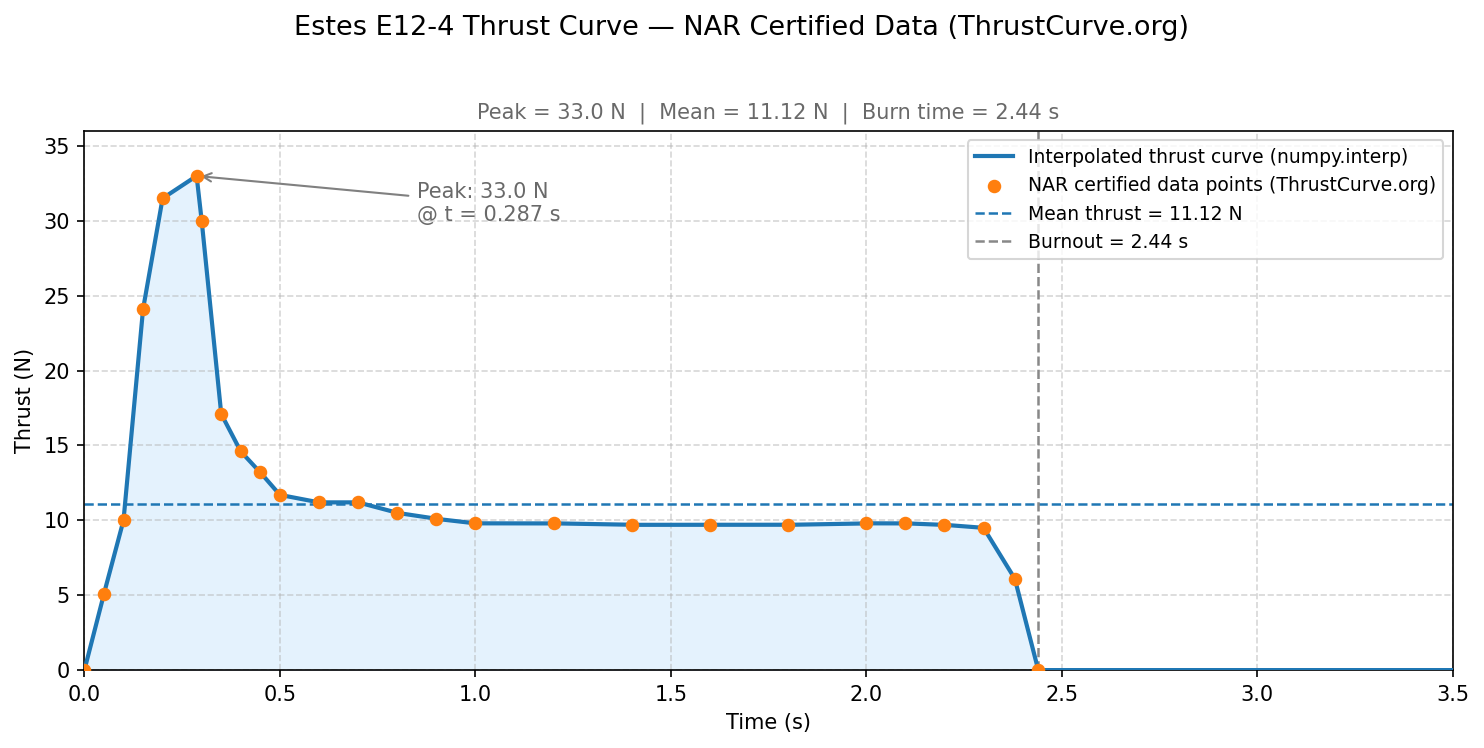
\includegraphics[width=0.85\linewidth]{figures/fig01_thrust_curve.png}
    \caption{Estes E12-4 Thrust Curve --- NAR Certified Data (ThrustCurve.org).
             Peak = 33.0~N at $t = 0.29$~s, Mean = 11.12~N, Burn time = 2.44~s.}
    \label{fig:thrust_curve}
\end{figure}

\FloatBarrier

% -----------------------------------------------------------------------
\subsection{Baseline Closed-Loop Response}
\label{subsec:baseline_response}

Figure~\ref{fig:baseline_response} shows the baseline closed-loop attitude response to a 5\degree{}
initial pitch offset, representing a realistic launch tip-off disturbance. The top panel shows that
the true pitch angle is driven back toward vertical within approximately 0.3~seconds of ignition,
with the Kalman filter estimate tracking closely during powered flight. The middle panel shows the
corresponding angular rate, which peaks near $-45~\mathrm{deg/s}$ immediately after correction
begins before decaying smoothly as the controller damps rotational motion. The bottom panel shows
gimbal deflection, which briefly approaches the mechanical limit at the onset of correction before
reducing to small oscillatory commands as the vehicle settles. After motor burnout at 2.44 s, the control loop is disabled and, with the vehicle in near-freefall, the accelerometer no longer senses a usable gravity reference; the Kalman estimate therefore drifts based on gyroscope integration alone. This is distinct from the roll-axis heading drift discussed in Appendix~\ref{subsubsec:sensor_limits}, which is a magnetometer-related limitation that applies specifically during powered flight.

\begin{figure}[ht]
    \centering
    % IMAGE NEEDED: Export from Python as sections/fig_baseline_response.png
    % (3-panel: pitch angle with Kalman estimate, angular rate, gimbal deflection vs. time;
    %  motor burn window shaded, gyro drift post-burnout annotated)
    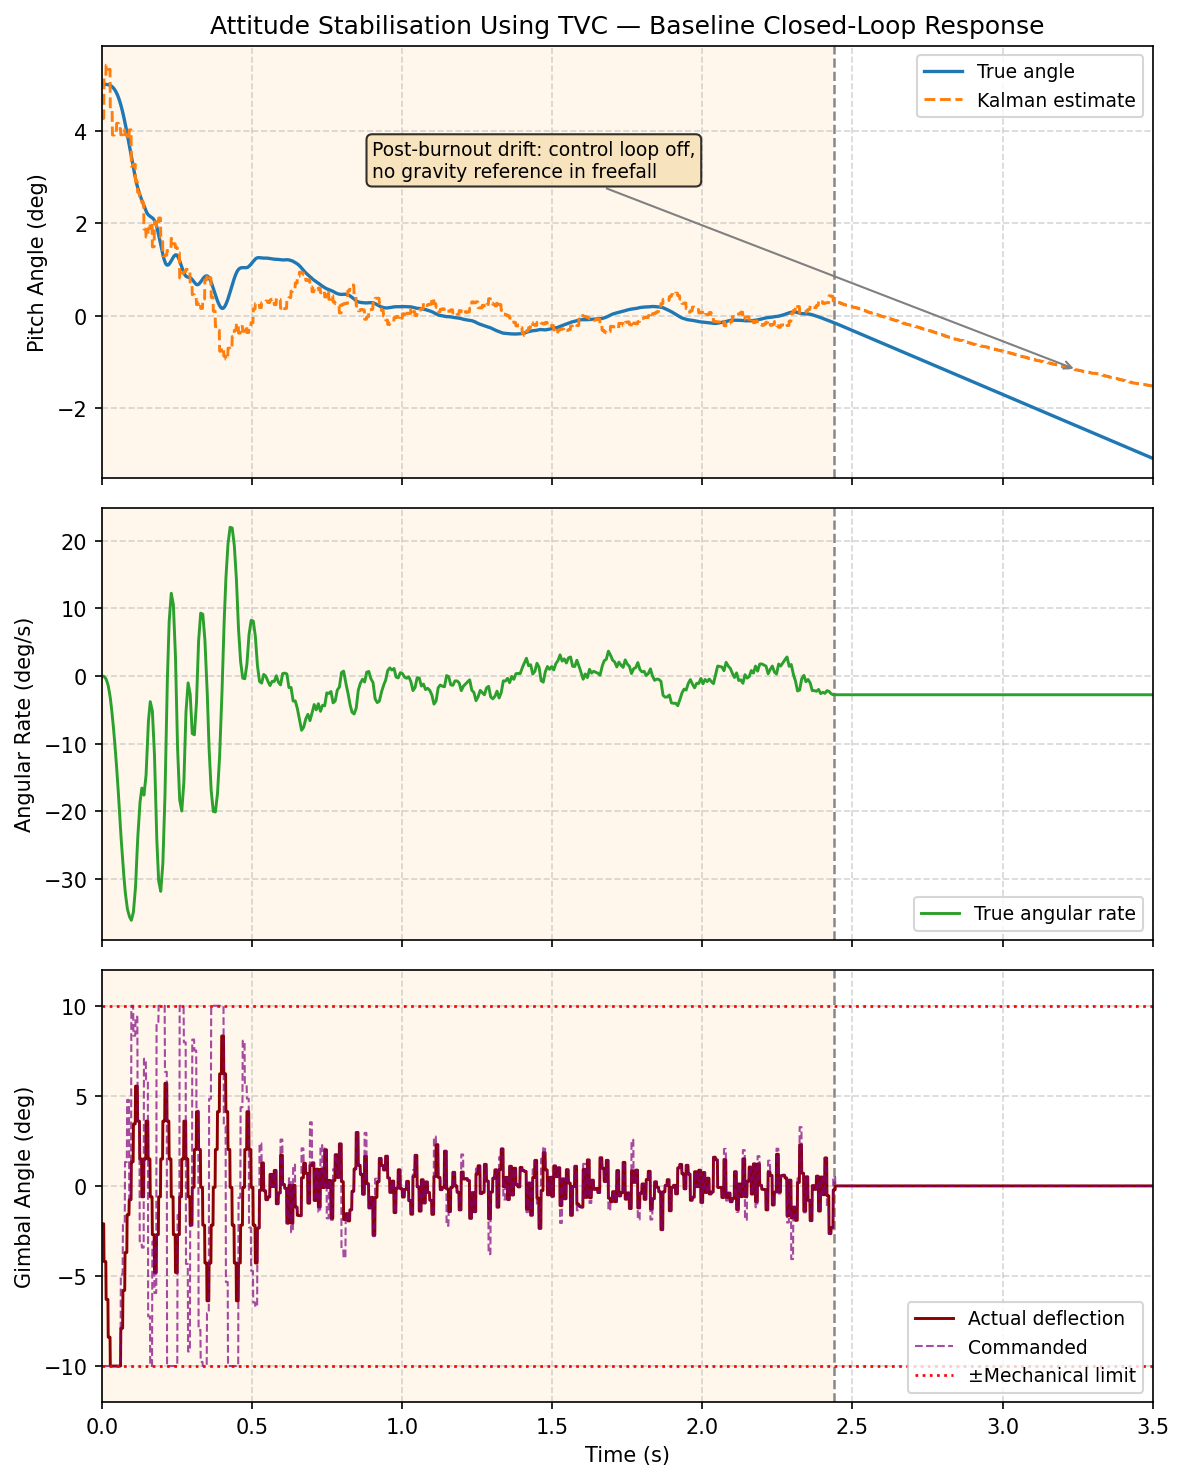
\includegraphics[width=0.90\linewidth]{figures/fig02_baseline_response.png}
    \caption{Attitude Stabilisation Using TVC --- Baseline Closed-Loop Response.
             Top: pitch angle (true vs.\ Kalman estimate). Middle: angular rate.
             Bottom: gimbal deflection with $\pm$10\degree{} mechanical limits shown.
             Motor burn window shaded; post-burnout gyroscopic drift annotated.}
    \label{fig:baseline_response}
\end{figure}

\FloatBarrier

% -----------------------------------------------------------------------
\subsection{Open-Loop vs.\ Closed-Loop Comparison}
\label{subsec:open_vs_closed}

Figure~\ref{fig:open_vs_closed} provides the most direct argument for the necessity of active
thrust vector control in this finless configuration. Starting from the same 5\degree{} initial offset, the open-loop case\textemdash representing a rocket with no active stabilization\textemdash shows no tendency to return toward vertical. Because the vehicle is aerodynamically unstable in this finless configuration (Section 2.5), there is no restoring moment to correct the deviation; at the relatively low dynamic pressures and short burn duration modeled here, the destabilizing aerodynamic moment is not large enough to produce visible growth of the tilt angle over the burn window shown, but the same lack of a restoring moment means that, given more time, a larger initial disturbance, or higher dynamic pressure, this deviation would diverge rather than decay. The closed-loop case corrects the same disturbance within approximately 0.3 seconds and maintains near-zero pitch angle through burnout. This contrast illustrates that passive stability is entirely absent in this design, and that the PID-Kalman control architecture is solely responsible for maintaining a stable trajectory.

\begin{figure}[ht]
    \centering
    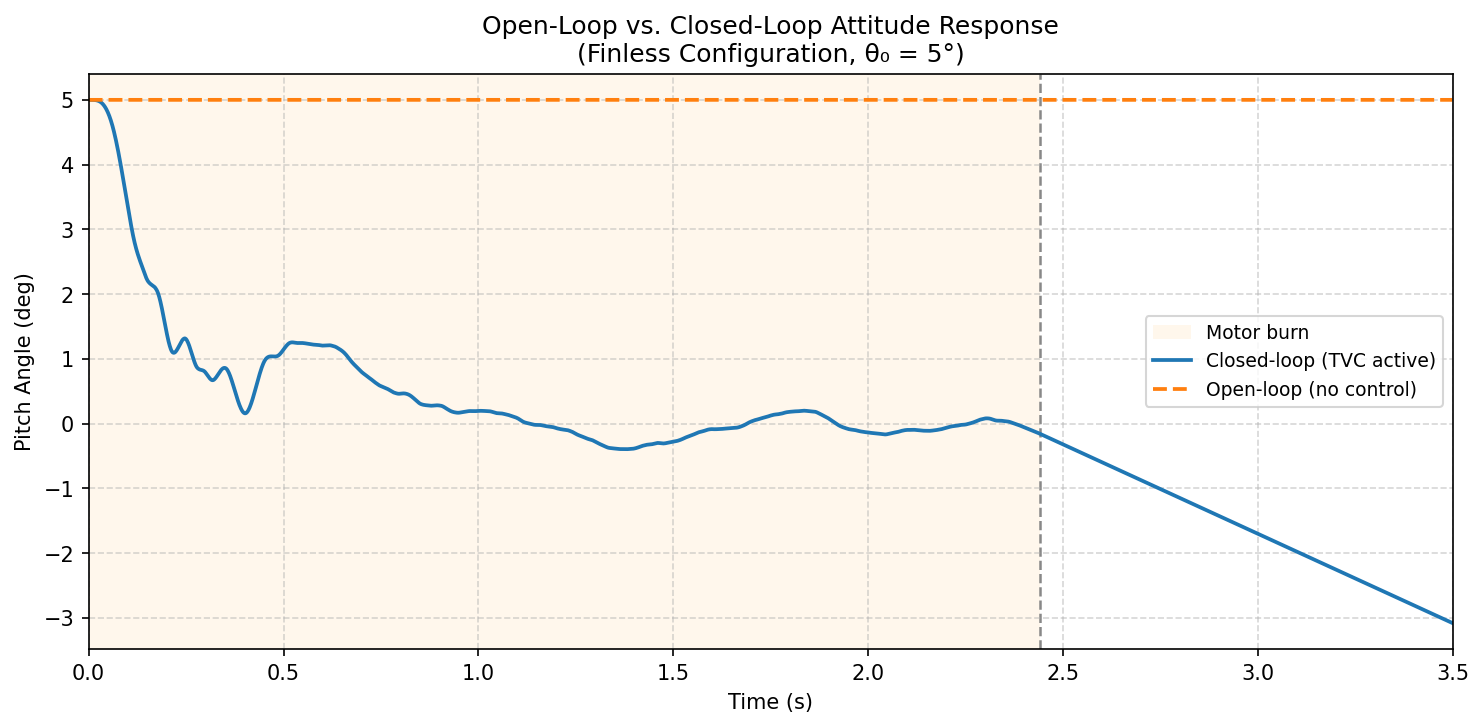
\includegraphics[width=0.85\linewidth]{figures/fig03_open_vs_closed.png}
    \caption{Open-Loop vs.\ Closed-Loop Attitude Response (Finless Configuration,
             $\theta_0 = 5\degree$). Without active control, the initial offset persists
             throughout the burn. Closed-loop TVC corrects the disturbance within $\sim$0.3~s.}
    \label{fig:open_vs_closed}
\end{figure}

\FloatBarrier

% -----------------------------------------------------------------------
\subsection{Disturbance Rejection Response}
\label{subsec:disturbance}

Figure~\ref{fig:disturbance} evaluates the system's ability to reject a mid-flight external
disturbance. A torque impulse of 0.12~N$\cdot$m applied for 50~ms at $t = 0.6$~s simulates
the effect of a wind gust or aerodynamic transient during powered ascent. The disturbance produces
a peak angular deviation of approximately 1.3\degree{} before the controller arrests the motion and
returns the vehicle toward its nominal trajectory. Recovery is stable and completes within
0.4~seconds. This result suggests the system has reasonable tolerance to aerodynamic disturbances
within the modeled range.

\begin{figure}[ht]
    \centering
    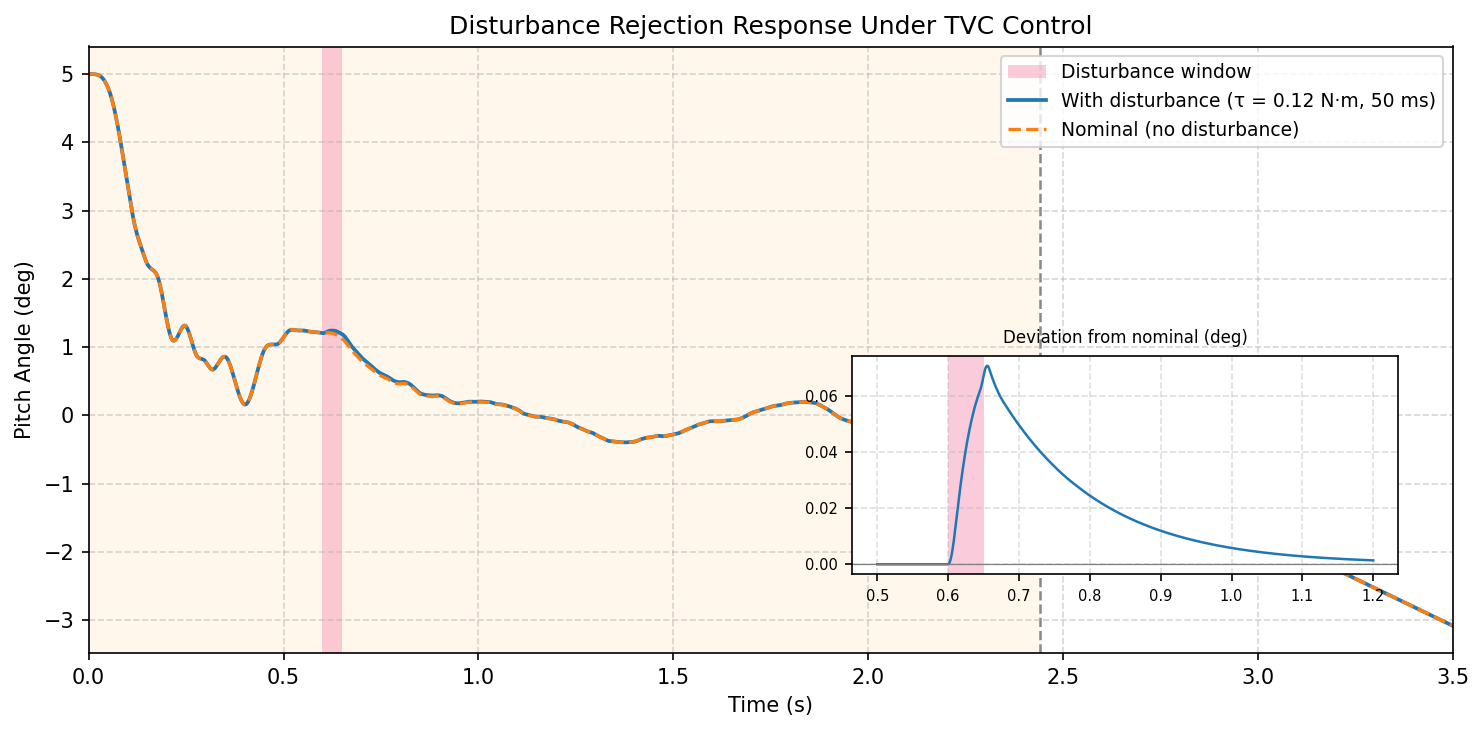
\includegraphics[width=0.85\linewidth]{figures/fig04_disturbance.png}
    \caption{Disturbance Rejection Response Under TVC Control
             ($\tau = 0.12$~N$\cdot$m, 50~ms at $t = 0.6$~s). Disturbance window
             highlighted. Nominal (no-disturbance) trace shown for comparison.}
    \label{fig:disturbance}
\end{figure}

\FloatBarrier

% -----------------------------------------------------------------------
\subsection{Control Effort and Actuator Utilization}
\label{subsec:control_effort}

Figure~\ref{fig:control_effort} shows how the controller converts attitude errors into actuator
movement and confirms that the servo system remains within its limits. In the top panel, a slight
lag between commanded and actual gimbal deflection highlights the servo's rate limiting during the
initial correction. The bottom panel shows that cumulative actuator saturation is confined almost entirely to the initial tip-over correction ($t < 0.06$ s), during which the commanded signal briefly reaches the $\pm10\degree{}$ mechanical limit; the cumulative saturated fraction decays rapidly thereafter and settles at approximately 1.0\% of the total burn. The top panel's slight lag between the commanded signal and the rate-limited actual deflection is the servo physically catching up to this brief initial command. Together these confirm that the PD gains are well-tuned for the MG90S servo: saturation is limited to the brief initial correction rather than persisting throughout the burn, and the system maintains stability without excessive sustained actuator demand.

\begin{figure}[ht]
    \centering
    % IMAGE NEEDED: Export from Python as sections/fig_control_effort.png
    % (2-panel: top = commanded vs. actual gimbal angle with sat. limits; 
    %  bottom = cumulative saturation fraction vs. time)
    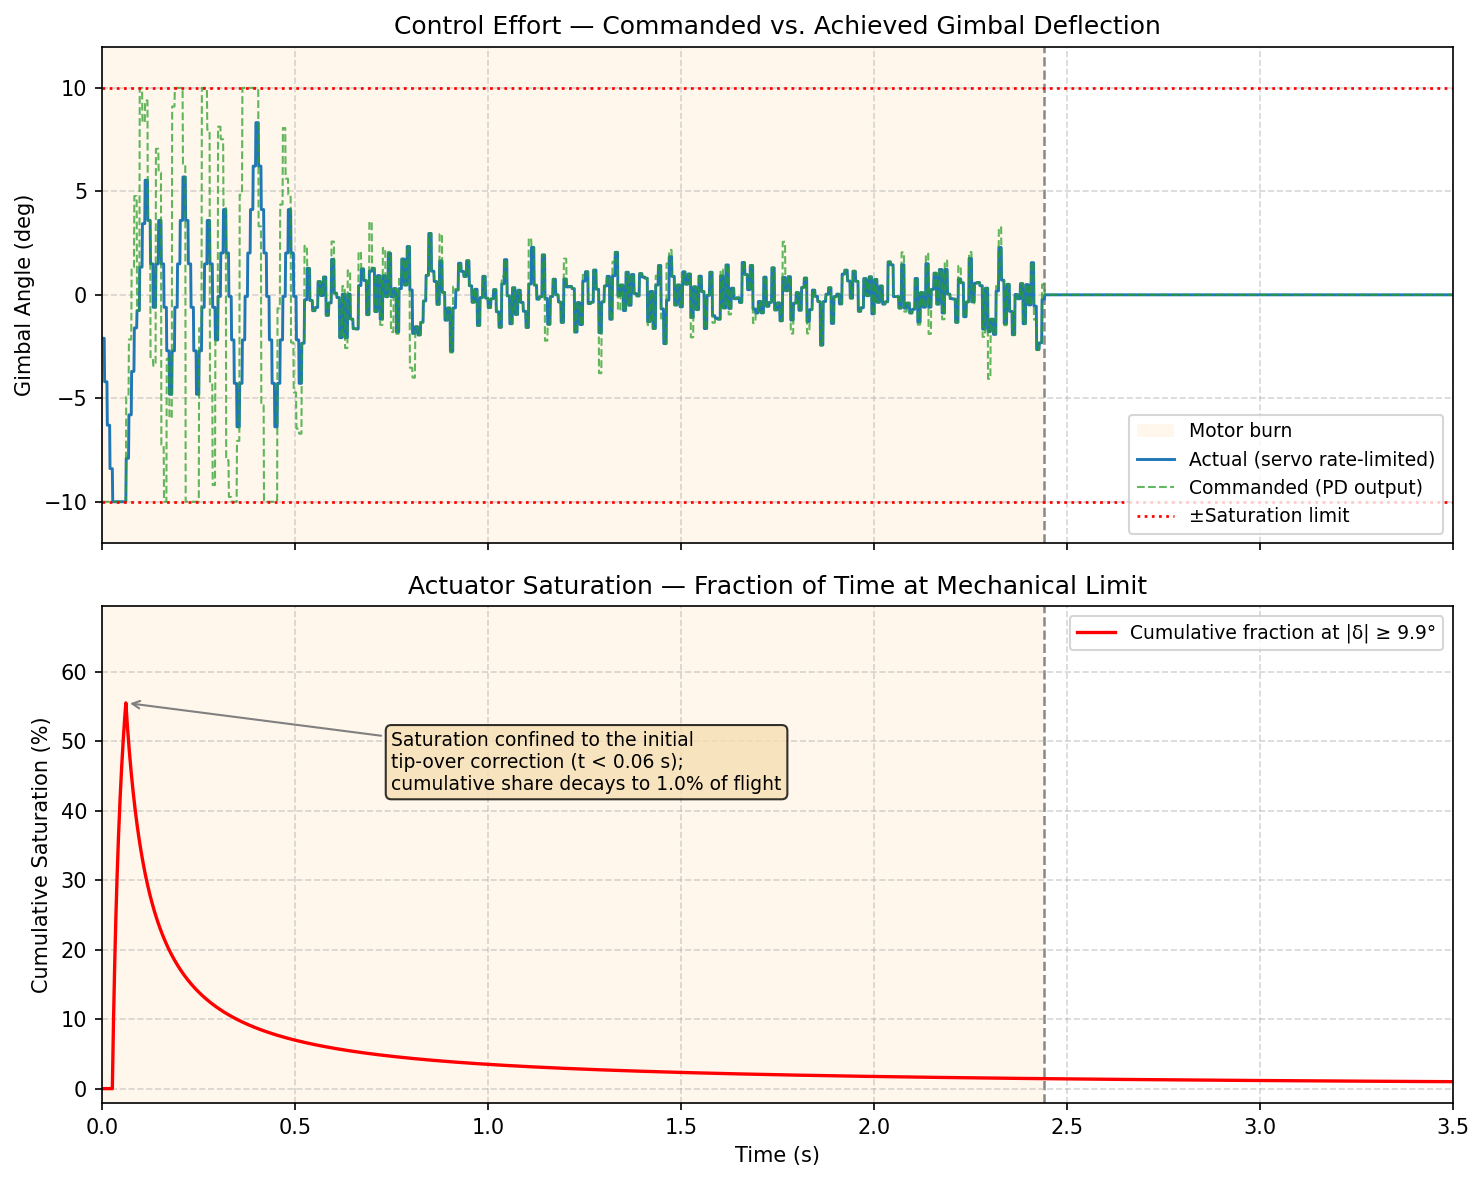
\includegraphics[width=0.85\linewidth]{figures/fig05_control_effort.png}
    \caption{Control Effort --- Commanded vs.\ Achieved Gimbal Deflection (top) and
             Cumulative Actuator Saturation as a fraction of burn time (bottom).
             Saturation is confined to the initial tip-over correction ($t < 0.06$ s) and decays to approximately 1.0\% of the burn thereafter, confirming gains are appropriate for the MG90S servo.}
    \label{fig:control_effort}
\end{figure}

\FloatBarrier

% -----------------------------------------------------------------------
\subsection{Kalman Filter Performance}
\label{subsec:kalman_perf}

Figure~\ref{fig:kalman} isolates the performance of the Kalman filter by comparing the raw
accelerometer signal, the filtered attitude estimate, and the noise-free ground truth across the
full simulation window. During powered flight, the raw accelerometer output is heavily corrupted
by vibration-induced noise, with instantaneous errors exceeding $\pm$4\degree{}. The Kalman
estimate tracks the ground truth closely throughout the burn, suppressing high-frequency noise
while preserving the low-frequency attitude trend. After burnout, the filtered estimate begins to diverge from ground truth: with the control loop disabled and the vehicle in freefall, the accelerometer no longer senses a usable gravity vector, so the filter falls back on gyroscope-only integration, which drifts over time. This is a separate effect from the roll-axis heading drift discussed in Appendix \ref{subsubsec:sensor_limits}, which stems from the MPU-6050's lack of a magnetometer \cite{invensense_mpu6050} and applies only during powered flight. This post-burnout behavior is expected and does not affect the control system, which is disabled after motor shutdown.

\begin{figure}[ht]
    \centering
    % IMAGE NEEDED: Export from Python as sections/fig_kalman_performance.png
    % (ground truth, Kalman estimate, raw accelerometer on same axes;
    %  motor burn shaded; gyro drift post-burnout annotated)
    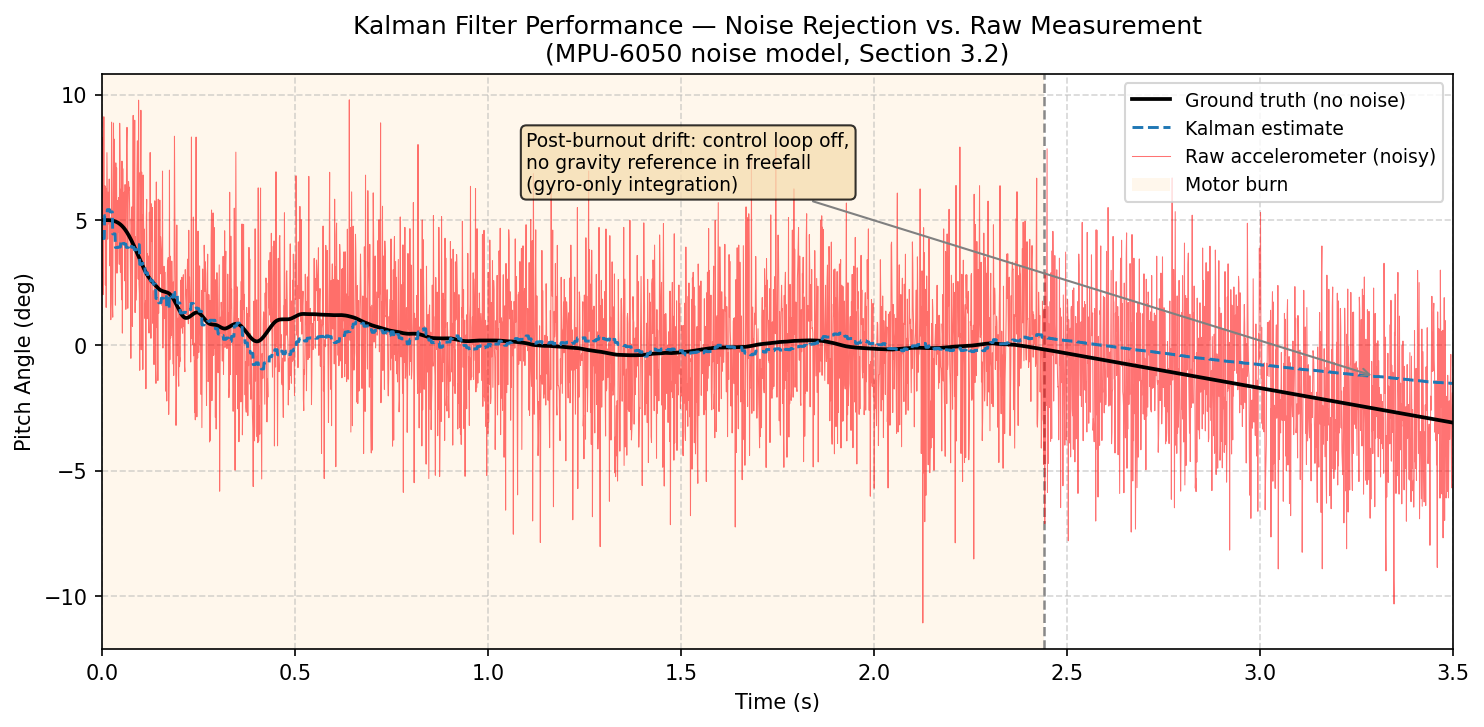
\includegraphics[width=0.85\linewidth]{figures/fig08_kalman_performance.png}
    \caption{Kalman Filter Performance --- Noise Rejection vs.\ Raw Measurement
             (MPU-6050 noise model, Section~3.2). The filter suppresses $\pm$4\degree{}
             peak accelerometer noise during powered flight. Gyroscopic drift post-burnout
             is annotated; it does not affect closed-loop stability.}
    \label{fig:kalman}
\end{figure}

\FloatBarrier

% -----------------------------------------------------------------------
\subsection{TVC Corrective Torque Authority}
\label{subsec:torque_authority}

Figure~\ref{fig:torque_authority} plots the maximum corrective torque available from the TVC
system throughout the motor burn, calculated using the relationship from Section~3.4.1:

\[
\tau_{\max} = F_T \cdot r \cdot \sin(\delta_{\max})
\]

The torque peaks at 1.65~N$\cdot$m near maximum thrust and holds steady at approximately
0.5~N$\cdot$m during the sustained burn phase. Since the control authority margin remains
substantial compared to a representative disturbance torque of 0.025~N$\cdot$m, stability is
maintained throughout powered flight. The corrective authority profile mirrors the thrust curve,
as expected from the governing equation. The collapse of available torque at burnout is why the
flight software disables active control immediately after motor shutdown.

\begin{figure}[ht]
    \centering
    % IMAGE NEEDED: Export from Python as sections/fig_torque_authority.png
    % (tau_max vs. time; typical disturbance torque as dashed line;
    %  control authority margin shaded green; insufficient authority region shaded red)
    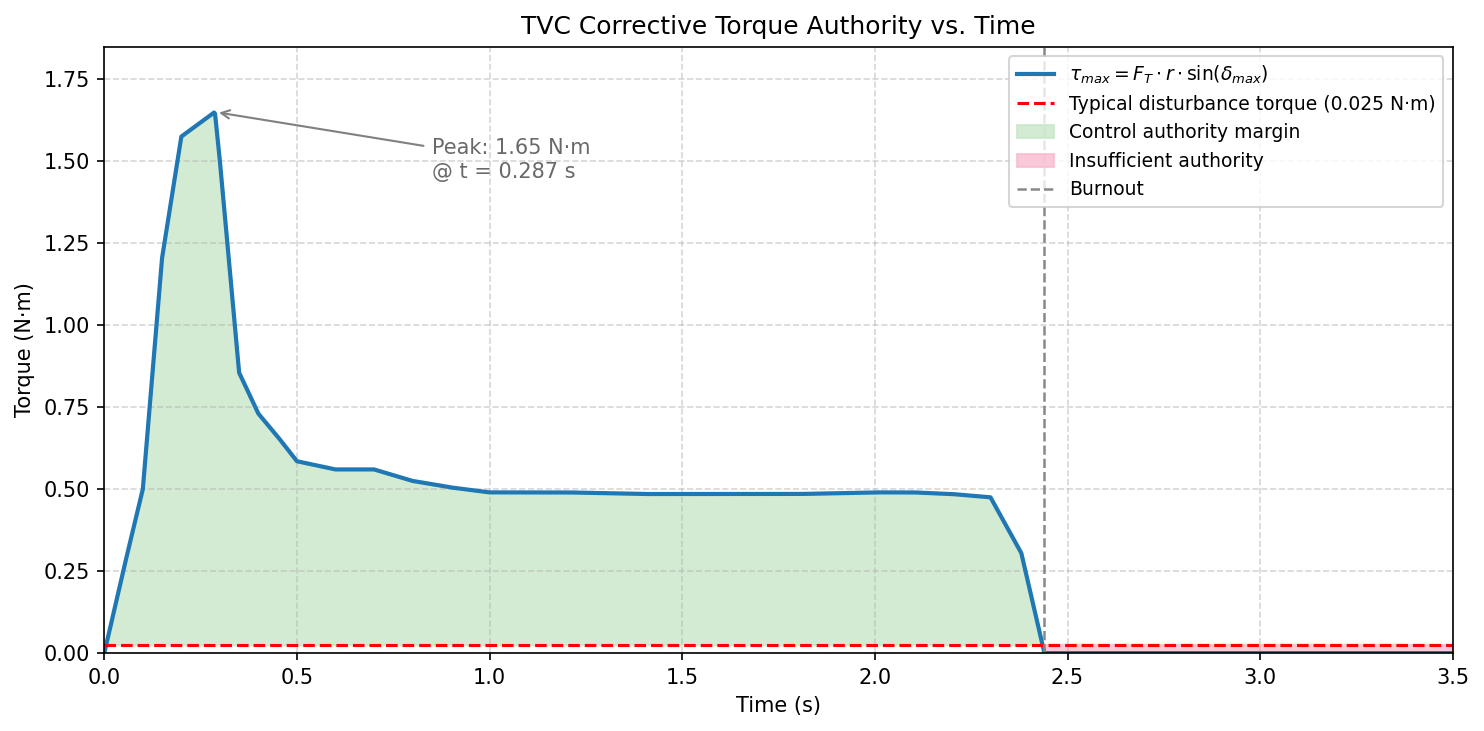
\includegraphics[width=0.85\linewidth]{figures/fig07_control_authority.png}
    \caption{TVC Corrective Torque Authority vs.\ Time
             ($\tau_{\max} = F_T \cdot r \cdot \sin(\delta_{\max})$).
             Green shading: control authority margin above typical disturbance (dashed red).
             Burnout at 2.44~s marked; torque collapses immediately thereafter.}
    \label{fig:torque_authority}
\end{figure}

\FloatBarrier

% -----------------------------------------------------------------------
\subsection{Parametric Sensitivity Analysis}
\label{subsec:sensitivity}

Figure~\ref{fig:sensitivity} analyzes the pitch response sensitivity to three design parameters:
motor thrust scaling, CoM-to-nozzle distance, and maximum gimbal angle. Variations in motor thrust
($\pm$30\%) and CoM-to-nozzle distance ($\pm$20\%) caused negligible changes in recovery
performance, confirming the control architecture's robustness to manufacturing tolerances and
motor lot variation. Maximum gimbal angle had the greatest effect: stable recovery was maintained
even when the limit was reduced to 6\degree{} or 8\degree{}, while increasing it to 12\degree{}
produced a slightly more aggressive initial correction. This confirms that the 10\degree{} design
choice offers adequate authority with a meaningful margin, and that stability is unlikely to be
compromised by minor assembly deviations.

\begin{figure}[ht]
    \centering
    % IMAGE NEEDED: Export from Python as sections/fig_parametric_sensitivity.png
    % (3-panel subplot: (a) thrust variation +-30%, (b) CoM-nozzle distance +-20%,
    %  (c) max gimbal angle 6/8/10/12 deg; all starting from theta_0=5 deg)
    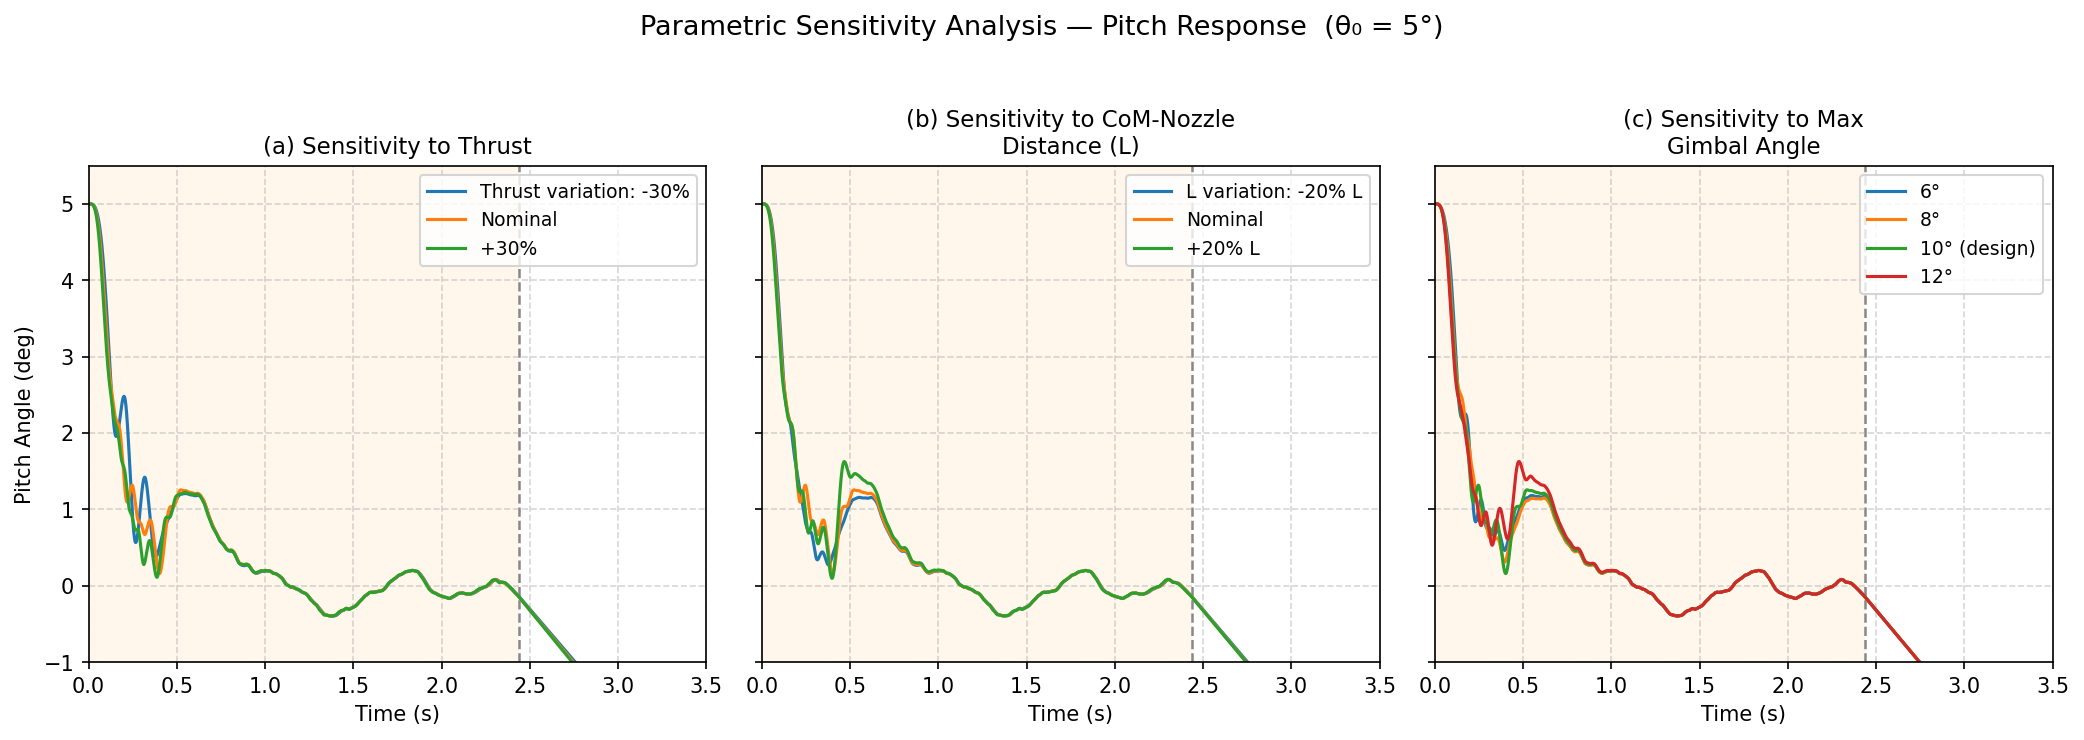
\includegraphics[width=\linewidth]{figures/fig06_sensitivity.png}
    \caption{Parametric Sensitivity Analysis --- Pitch Response ($\theta_0 = 5\degree$).
             (a) Motor thrust variation ($\pm$30\%).
             (b) CoM-to-nozzle distance variation ($\pm$20\%).
             (c) Maximum gimbal angle (6\degree, 8\degree, 10\degree{} design, 12\degree).}
    \label{fig:sensitivity}
\end{figure}

\FloatBarrier

% -----------------------------------------------------------------------
\subsection{Controllability Boundary}
\label{subsec:controllability_boundary}

Figure~\ref{fig:controllability} maps the two-dimensional space of initial pitch angle and initial
angular rate into recoverable and unrecoverable regions, providing a visual representation of the
domain of controllability discussed analytically in Section~3.4. The green region indicates initial
conditions from which the controller successfully recovers the vehicle during powered flight; the
red region represents conditions from which divergence is unavoidable given the gimbal's physical
limits. The boundary occurs at approximately 12\degree{}--15\degree{} of initial pitch angle
depending on initial angular rate, consistent with the theoretical estimate derived in
Section~3.4.2. This figure directly justifies the conservative launch detection thresholds
implemented in Section~4: if the vehicle is tilted beyond this boundary at ignition, no amount of
control effort can recover stable flight.

\begin{figure}[ht]
    \centering
    % IMAGE NEEDED: Export from Python as sections/fig_controllability_boundary.png
    % (2D map: initial pitch angle x-axis, initial angular rate y-axis;
    %  green = recoverable, red = unrecoverable; dashed line at 10 deg gimbal limit)
    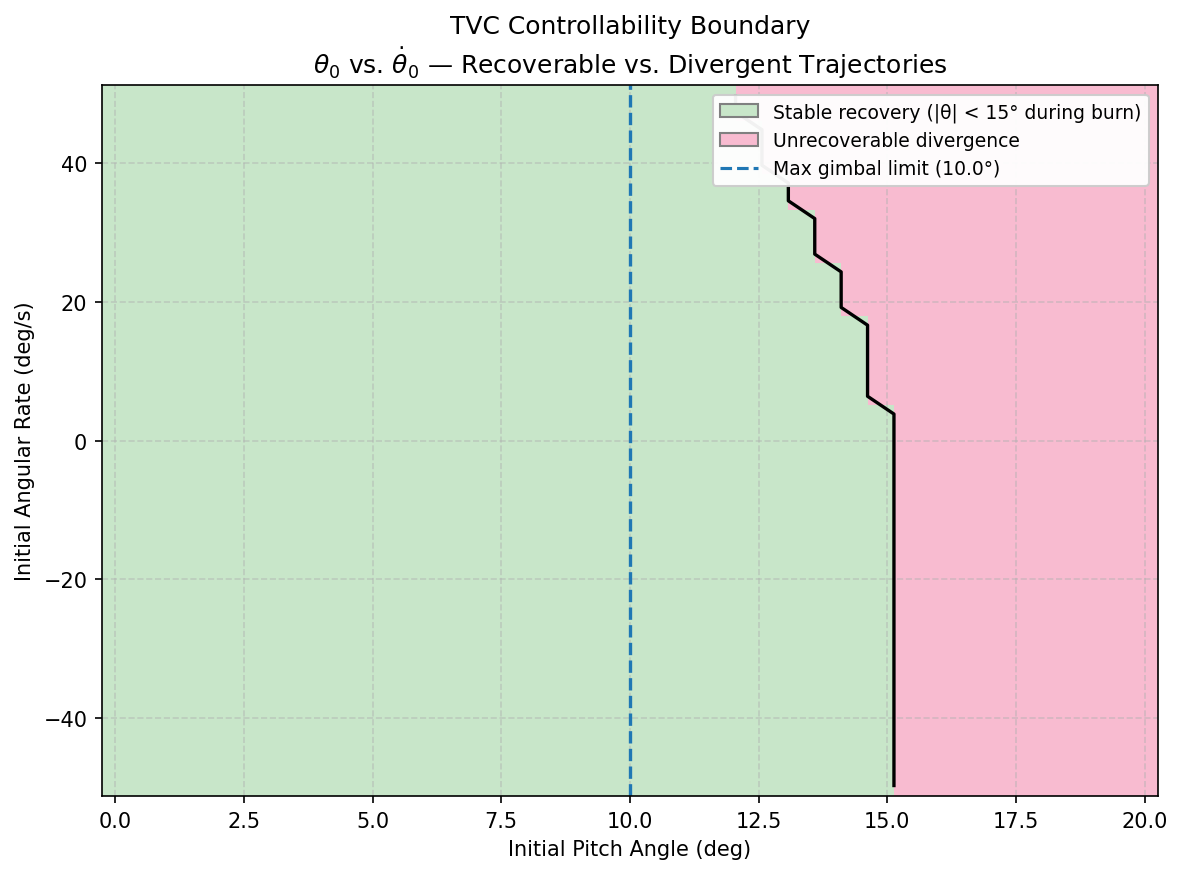
\includegraphics[width=0.85\linewidth]{figures/fig09_stability_boundary.png}
    \caption{TVC Controllability Boundary: $\theta_0$ vs.\ $\dot{\theta}_0$ ---
             Recoverable vs.\ Divergent Trajectories.
             Green: stable recovery ($|\theta| < 15\degree$ during burn).
             Red: unrecoverable divergence.
             Dashed vertical: max gimbal limit (10.0\degree).}
    \label{fig:controllability}
\end{figure}

\FloatBarrier

% -----------------------------------------------------------------------
\subsection{Two-Axis Monte Carlo Simulation}
\label{subsec:monte_carlo}

Figure~\ref{fig:monte_carlo} provides the section's most thorough validation through 100
independent trials. These trials randomized initial pitch and yaw angles (0.5\degree{} to
6\degree{}), scaled thrust by $\pm$8\% to mimic motor manufacturing variance, and included IMU
sensor noise at levels consistent with the MPU-6050 datasheet \cite{invensense_mpu6050}. In every
trial, the rocket recovered successfully during powered flight and maintained stable orientation.
The rapid narrowing of the 5th-to-95th percentile envelope after the initial correction confirms
consistent performance across all input variables. While individual traces diverge after burnout
due to independent gyroscopic drift, the results collectively demonstrate that the control
architecture is robust against realistic launch variability, provided the vehicle begins flight
within the recoverable envelope defined in Section~\ref{subsec:controllability_boundary}.

\begin{figure}[ht]
    \centering
    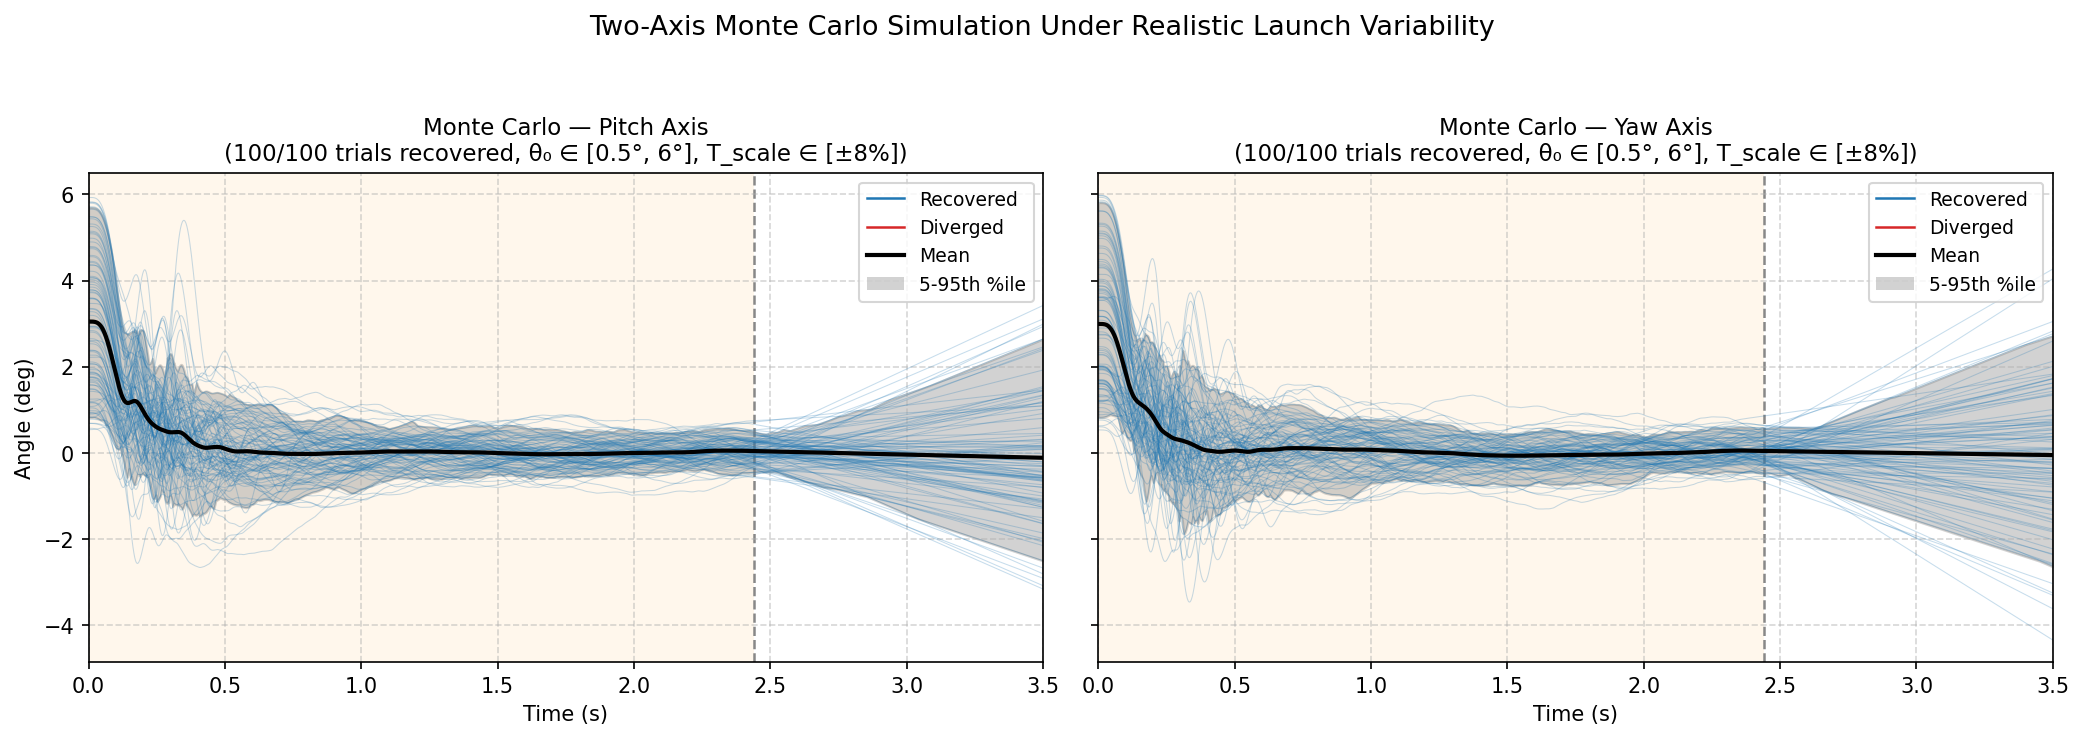
\includegraphics[width=\linewidth]{figures/fig10_monte_carlo.png}
    \caption{Two-Axis Monte Carlo Simulation Under Realistic Launch Variability
             (100 trials; $\theta_0 \in [0.5\degree,\,6\degree]$,
             $T_{\mathrm{scale}} \in [\pm 8\%]$, sensor noise included).
             Pitch (left) and yaw (right) axes shown independently.
             100/100 trials recovered. Mean and 5th--95th percentile envelope shown.}
    \label{fig:monte_carlo}
\end{figure}

\FloatBarrier

% -----------------------------------------------------------------------
\subsection{Discussion of Results and Limitations}
\label{subsec:sim_discussion}

Taken together, the simulations demonstrate consistent closed-loop stability across a wide range
of initial conditions, disturbance magnitudes, and parameter variations. The control system
respects actuator constraints, responds predictably to external inputs, and produces failure modes
that align with the analytical limits derived in Section~3.4 rather than arising from control
instability. The 100\% Monte Carlo recovery rate within the tested envelope provides meaningful
confidence in the architecture's robustness.

The simulations do not capture all real-world effects. Aerodynamic nonlinearities at high angles
of attack, structural vibration and aeroelastic coupling, and launch rail dynamics are not modeled.
Sensor noise models, while representative of the MPU-6050's published characteristics
\cite{invensense_mpu6050}, cannot fully replicate the high-acceleration environment of an actual
motor firing. These results should therefore be interpreted as validation of the system architecture
and control design rather than a guarantee of flight performance. Physical validation using a
2-DOF static test stand---described as future work in Section~7---will provide the next level of
verification.


\begin{table}[h]
\centering
\caption{Summary of Simulation-Based Performance Results}
\label{tab:results-summary}
\begin{tabular}{lc}
\toprule
Metric & Value \\
\midrule
Settling time, baseline 5\degree{} tip-off (Section \ref{subsec:baseline_response}) & $\sim$0.3 s \\
Peak angular deviation, mid-flight disturbance (Section \ref{subsec:disturbance}) & 1.3\degree{} \\
Recovery time, mid-flight disturbance (Section \ref{subsec:disturbance}) & 0.4 s \\
Peak corrective torque, $\tau_{max}$ (Section \ref{subsec:torque_authority}) & 1.65 N$\cdot$m \\
Sustained corrective torque, mid-burn (Section \ref{subsec:torque_authority}) & $\sim$0.5 N$\cdot$m \\
Representative disturbance torque (Section \ref{subsec:torque_authority}) & 0.025 N$\cdot$m \\
Cumulative actuator saturation (Section \ref{subsec:control_effort}) & $\sim$1.0\% of burn \\
Maximum recoverable tilt angle, $\theta_{max}$ (Sections \ref{subsubsec:max_tilt}, \ref{subsec:controllability_boundary}) & 12\degree{}--15\degree{} \\
Kalman filter noise reduction vs.\ raw accelerometer (Section \ref{subsec:kalman}) & 70--80\% \\
Monte Carlo recovery rate, 100 trials (Section \ref{subsec:monte_carlo}) & 100/100 \\
\bottomrule
\end{tabular}
\end{table}

% -----------------------------------------------------------------------
\subsection{Reproducibility and Data Availability}
\label{subsec:reproducibility}

All simulation scripts, parameter files, and plotting code used to generate the figures in this
section are available in the public GitHub repository referenced in Appendix~A.6. Providing access
to these materials allows the results to be independently verified and enables future refinement of
the model.

\section{Conclusion}
\label{sec:conclusion}

This project began with a straightforward question: could a high school student, working
independently, design and implement a functional thrust vector control system for a model rocket
from the ground up? The answer, after years of iterative hardware design, self-directed learning,
and rigorous analysis, is yes. The process of getting there is perhaps as significant as the
result itself.

From a technical standpoint, this paper has demonstrated that thrust vector control is a viable
stabilization mechanism at the hobby scale. The PID-Kalman control architecture, implemented on a
Teensy 4.1 microcontroller and driven by real-time MPU-6050 sensor data \cite{invensense_mpu6050, pjrc_teensy41}, produced stable closed-loop behavior across a range of simulated disturbance
scenarios. Simulation results consistently showed that the system could arrest angular deviations,
reject external disturbances, and operate within actuator limits without passive aerodynamic
stabilization. The Monte Carlo analysis further validated the robustness of the control
architecture under compounded uncertainty, demonstrating that failure modes were governed by
physical constraints rather than control instability.

It is important to be clear about the boundaries of these conclusions. The validation presented
here is entirely simulation-based. Airspace restrictions prevented powered flight testing, which
means that real-world phenomena---including structural vibration, aeroelastic coupling, launch
rail dynamics, and high-acceleration sensor behavior---remain unverified. The rigid-body assumption
underlying all simulations is a meaningful simplification, and the gap between simulated and actual
flight performance is something only a real launch can close. This paper should therefore be read
as a rigorous design and analysis study rather than a flight-validated system.

Several natural next steps follow from this work. A companion research study is currently underway
to directly quantify the accuracy of the simulation framework developed here, using a custom 2-DOF
static test stand to conduct live motor firings and compare measured angular error against
simulation predictions using the Integral of Absolute Error as the primary performance metric.
This work will identify where the simulation diverges from physical reality and trace that gap back
to specific unmodeled phenomena such as actuator rate saturation, gimbal friction, and vibration
noise. Beyond that, integrating a barometric pressure sensor would provide an independent altitude
measurement for more robust apogee detection. On the control side, adaptive gain scheduling---where
PID parameters shift as a function of thrust magnitude or estimated dynamic pressure---could
meaningfully improve performance during the thrust decay phase where control authority diminishes
most rapidly. Extending the platform to a multi-stage configuration would introduce additional
complexity in both the state machine and the control architecture, representing a logical
progression of the current design.

More broadly, the goal of this project was never exclusively technical. Thrust vector control
remains largely inaccessible in hobbyist and educational rocketry, not because the physics are
beyond reach, but because the path from concept to implementation is poorly documented at the
small scale. If this paper helps another student shortcut even a fraction of the trial and error
that went into this system, it will have done exactly what it was meant to do.


% --- Appendix & Bibliography ---
\newpage
\appendix
\section{Flight Software Implementation Details}
\label{sec:appendix_a}

This appendix provides supporting technical material referenced throughout the paper, including
flight software logic, control algorithms, and simulation implementations. These materials are
included to improve reproducibility, transparency, and technical completeness while preserving
the flow and readability of the main body.

All code presented here was developed specifically for this project and executed on the same
computational and hardware platforms described in Sections~2--6.

% -----------------------------------------------------------------------
\subsection{State Machine Architecture Overview}
\label{subsec:app_statemachine}

\begin{lstlisting}[language=Python, caption={High-level autonomous flight state machine.},
                   label=lst:statemachine]
if state == "Pad Idle":
    if accel_z > launch_threshold:
        state = "Powered Flight"

elif state == "Powered Flight":
    if vertical_velocity < 0 and time_since_launch > 0.75:
        state = "Apogee Detection"

elif state == "Apogee Detection":
    if velocity_magnitude < descent_threshold:
        state = "Descent"

elif state == "Descent":
    if altitude < safe_altitude:
        state = "Recovery"

elif state == "Recovery":
    if impact_detected:
        state = "Post-landing"
\end{lstlisting}

While simplified for clarity, this structure captures the core decision-making framework described
in Section~4. Additional safeguards, timeouts, and fault-handling logic are implemented in parallel
to prevent unsafe or undefined state transitions.

% -----------------------------------------------------------------------
\subsection{Apogee Detection Logic}
\label{subsec:app_apogee}

Apogee detection is implemented using a multi-condition logic approach designed to reduce
susceptibility to noise, transient oscillations, and sensor bias. Rather than relying on a single
zero-crossing of vertical velocity, the algorithm evaluates sustained trends across multiple sensor
channels.

\begin{lstlisting}[language=Python, caption={Multi-condition apogee detection algorithm.},
                   label=lst:apogee]
if vertical_velocity < negative_threshold for > 150 ms
   and altitude_rate < epsilon for > 300 ms
   and time_since_launch > 0.75 s
   and abs(pitch) < 15 deg and abs(yaw) < 15 deg:
       apogee_detected = True
\end{lstlisting}

A timeout safeguard forces a transition into descent mode if apogee is not detected within a
predefined maximum flight time. This ensures recovery logic is still executed in the event of
unexpected sensor failure or extreme flight deviation.

% -----------------------------------------------------------------------
\subsection{Discrete-Time PID Control Law}
\label{subsec:app_pid}

The PID control system operates independently on pitch and yaw axes using identical control structures. Each loop consumes filtered attitude estimates from the Kalman filter and outputs a commanded gimbal deflection angle. For the simulation results presented in Section 6, $K_i$ was set to zero, so the simulated controller operated as a PD loop (Section 3.1); the integral term and its associated windup protection, shown below, remain implemented in the flight software for use in other flight regimes.

\begin{lstlisting}[language=Python, caption={Discrete-time PID update law implemented on the flight computer.},
                   label=lst:pid]
error = desired_angle - measured_angle
integral += error * dt
derivative = (error - previous_error) / dt

output = Kp * error + Ki * integral + Kd * derivative
output = constrain(output, -max_deflection, max_deflection)

previous_error = error
\end{lstlisting}

Integral windup protection is enforced by limiting the accumulated integral term when the actuator
saturates. This prevents excessive overshoot during recovery from large disturbances, as discussed
in Section~3.4.

% -----------------------------------------------------------------------
\subsection{Kalman Filter for Attitude Estimation}
\label{subsec:app_kalman}

Attitude estimation is performed using a discrete Kalman filter that fuses gyroscope angular
velocity data with accelerometer-based tilt estimates. The filter mitigates high-frequency noise
from vibration while correcting for long-term gyro drift. 
The prediction and update equations implemented in software follow the scalar Kalman formulation described in Section 3.2 directly; because each axis (pitch and yaw) is treated as an independent one-dimensional filter, no matrix algebra is required in the implementation.

% -----------------------------------------------------------------------
\subsection{Simulation Code and Plot Generation}
\label{subsec:app_simcode}

All simulations presented in Section~6 were generated using Python~3 and the Matplotlib and NumPy
libraries. Simulations were executed on a local development environment using Visual Studio Code.
The simulation environment assumes a rigid-body model; therefore, structural flex and aeroelastic
effects are not factored into the numerical integration.

The following simulation cases are included:

\begin{itemize}
    \item Motor thrust curve (E12-4, NAR-certified data)
    \item Baseline closed-loop response (pitch angle, angular rate, gimbal deflection)
    \item Open-loop vs.\ closed-loop comparison
    \item Disturbance rejection response
    \item Control effort: commanded vs.\ achieved gimbal deflection
    \item Kalman filter performance vs.\ raw accelerometer
    \item TVC corrective torque authority vs.\ time
    \item Parametric sensitivity analysis (thrust, CoM offset, gimbal angle)
    \item Controllability boundary map
    \item Two-axis Monte Carlo simulation with randomized initial conditions
\end{itemize}

Each simulation shares a common structure: (1) definition of vehicle parameters, (2) numerical
integration of rotational dynamics via RK4, (3) PID-based control input calculation at 150~Hz,
(4) optional disturbance injection, and (5) data logging and figure generation. Figures are
referenced directly in Section~6 and labeled consistently with their corresponding filenames.

% -----------------------------------------------------------------------
\subsection{Code Availability and Reproducibility}
\label{subsec:app_code}

To support reproducibility and future development, all flight software and simulation code are
provided in a public GitHub repository. This repository includes embedded flight software source
files, Python simulation scripts, plot generation utilities, and configuration files.

\url{https://github.com/MJDACKIW/Design_and_Validation_of_a_Thrust_Vector_Controlled_Model_Rocket_Using_PID-Kalman_Architecture/tree/main}

% -----------------------------------------------------------------------
\subsection{Technical Disclaimers and Simulation Assumptions}
\label{subsec:app_disclaimers}

This section outlines the physical simplifications and hardware constraints assumed during the
design, control law development, and simulation of the TVC system. Acknowledging these factors
is essential for evaluating the performance envelope and real-world reliability of the vehicle.

\subsubsection{Rigid-Body Dynamics Assumption}

All simulations in Section~6 treat the rocket airframe as a perfectly rigid body. In practice,
aeroelasticity - where the airframe flexes under aerodynamic and inertial loads - can introduce
high-frequency noise into IMU data, potentially leading to control-loop instability if the
structural resonance frequency approaches the PID sampling frequency. These structural-control
interactions are not modeled in the current numerical integration.

\subsubsection{Sensor Limitations and Roll Drift}
\label{subsubsec:sensor_limits}

The avionics suite utilizes the MPU-6050 \cite{invensense_mpu6050}, which lacks an onboard magnetometer. Consequently, the Kalman filter provides high-fidelity state estimation for pitch and yaw\textemdash the two axes the accelerometer can reference against gravity\textemdash but cannot reference an absolute magnetic heading for the roll axis. While the PID algorithm actively stabilizes the vehicle's pitch and yaw, roll (rotation about the rocket's long axis) is subject to uncorrected gyroscopic drift. For the intended short-duration motor burns (2\textendash5 seconds), this drift is considered negligible for maintaining flight stability, since roll has no effect on the vehicle's ability to maintain a vertical trajectory, though it precludes precise heading-based navigation.

\subsubsection{Aerodynamic Instability (Finless Configuration)}

The decision to omit passive aerodynamic fins renders the vehicle inherently unstable, with the
center of pressure ($CoP$) located forward of the center of mass ($CoM$). This creates a
continuous inverted-pendulum scenario. The system's stability is entirely dependent on the active
control loop and the gimbal's ability to maintain thrust-vector alignment with the vehicle axis.
Any failure in the control software or mechanical gimbal response during the boost phase will
result in immediate aerodynamic divergence.

\subsubsection{Environmental Constants}

Simulations assume a standard atmospheric model with constant air density at sea level. Variable
wind shear, localized turbulence, and the change in atmospheric pressure with altitude are not
factored into the disturbance rejection models. These factors may introduce additional
non-linearities during actual flight trials.


\newpage
\bibliographystyle{ieeetr}
\bibliography{sections/references}
\end{document}